\numberwithin{equation}{section}
\numberwithin{figure}{section}
\numberwithin{table}{section}

\subsection{Cohort Information}
\label{apd:cohort_information}
To provide further context about the temporal structure and adherence dynamics in our cohort, in Figure~\ref{fig:data_overview}, we include illustrative visualizations of a representative patient timeline and the operational definition of medication adherence. 
Figure~\ref{fig:patient_trajectory} shows an example trajectory of schizophrenia patient in our study, highlighting the structure of monthly adherence (adherent vs. non-adherent), the snapshot time \(\tau\) used for prediction, and the timing of the first observed adverse event, defined as the earliest occurrence of involuntary hospitalization, jail booking, or premature death. 
This figure illustrates how patient histories are segmented, how time-to-event is defined from the prediction snapshot, and the types of adverse outcomes we consider.
Figure~\ref{fig:adherence_indicator} illustrates how monthly medication adherence is binarized. 
Daily prescription coverage is computed based on refill history, and a patient-month is labeled non-adherent if medication availability covers 10 days or fewer. 
(For medications prescribed at different frequencies, such as weekly, adherence is defined analogously based on the number of covered doses within the month).
The choice of this threshold is discussed in Appendix~\ref{apd:cohort_nonadherence}.
These binarized monthly non-adherence indicators serve as time-varying covariates in our dataset.
Together, these visualizations clarify the temporal modeling setup, the construction of key covariates, and how the outcome is defined in our survival analysis framework.

\begin{figure*}[thb]
\floatconts
  {fig:data_overview}
  {\caption{Overview of Schizophrenia Patient Trajectory in Allegheny County. (a) We look at the timing of the first composite outcome \(\in \{\text{\textcolor{orange}{Involuntary Hospitalization}, \textcolor{red}{Jail Stay}, \textbf{Death}}\}\). (b) Non-adherence at each month is calculated by looking at the daily equivalence of prescribed refills available for each month.}}
  {%
    \subfigure[Patient Trajectory]{\label{fig:patient_trajectory}%
      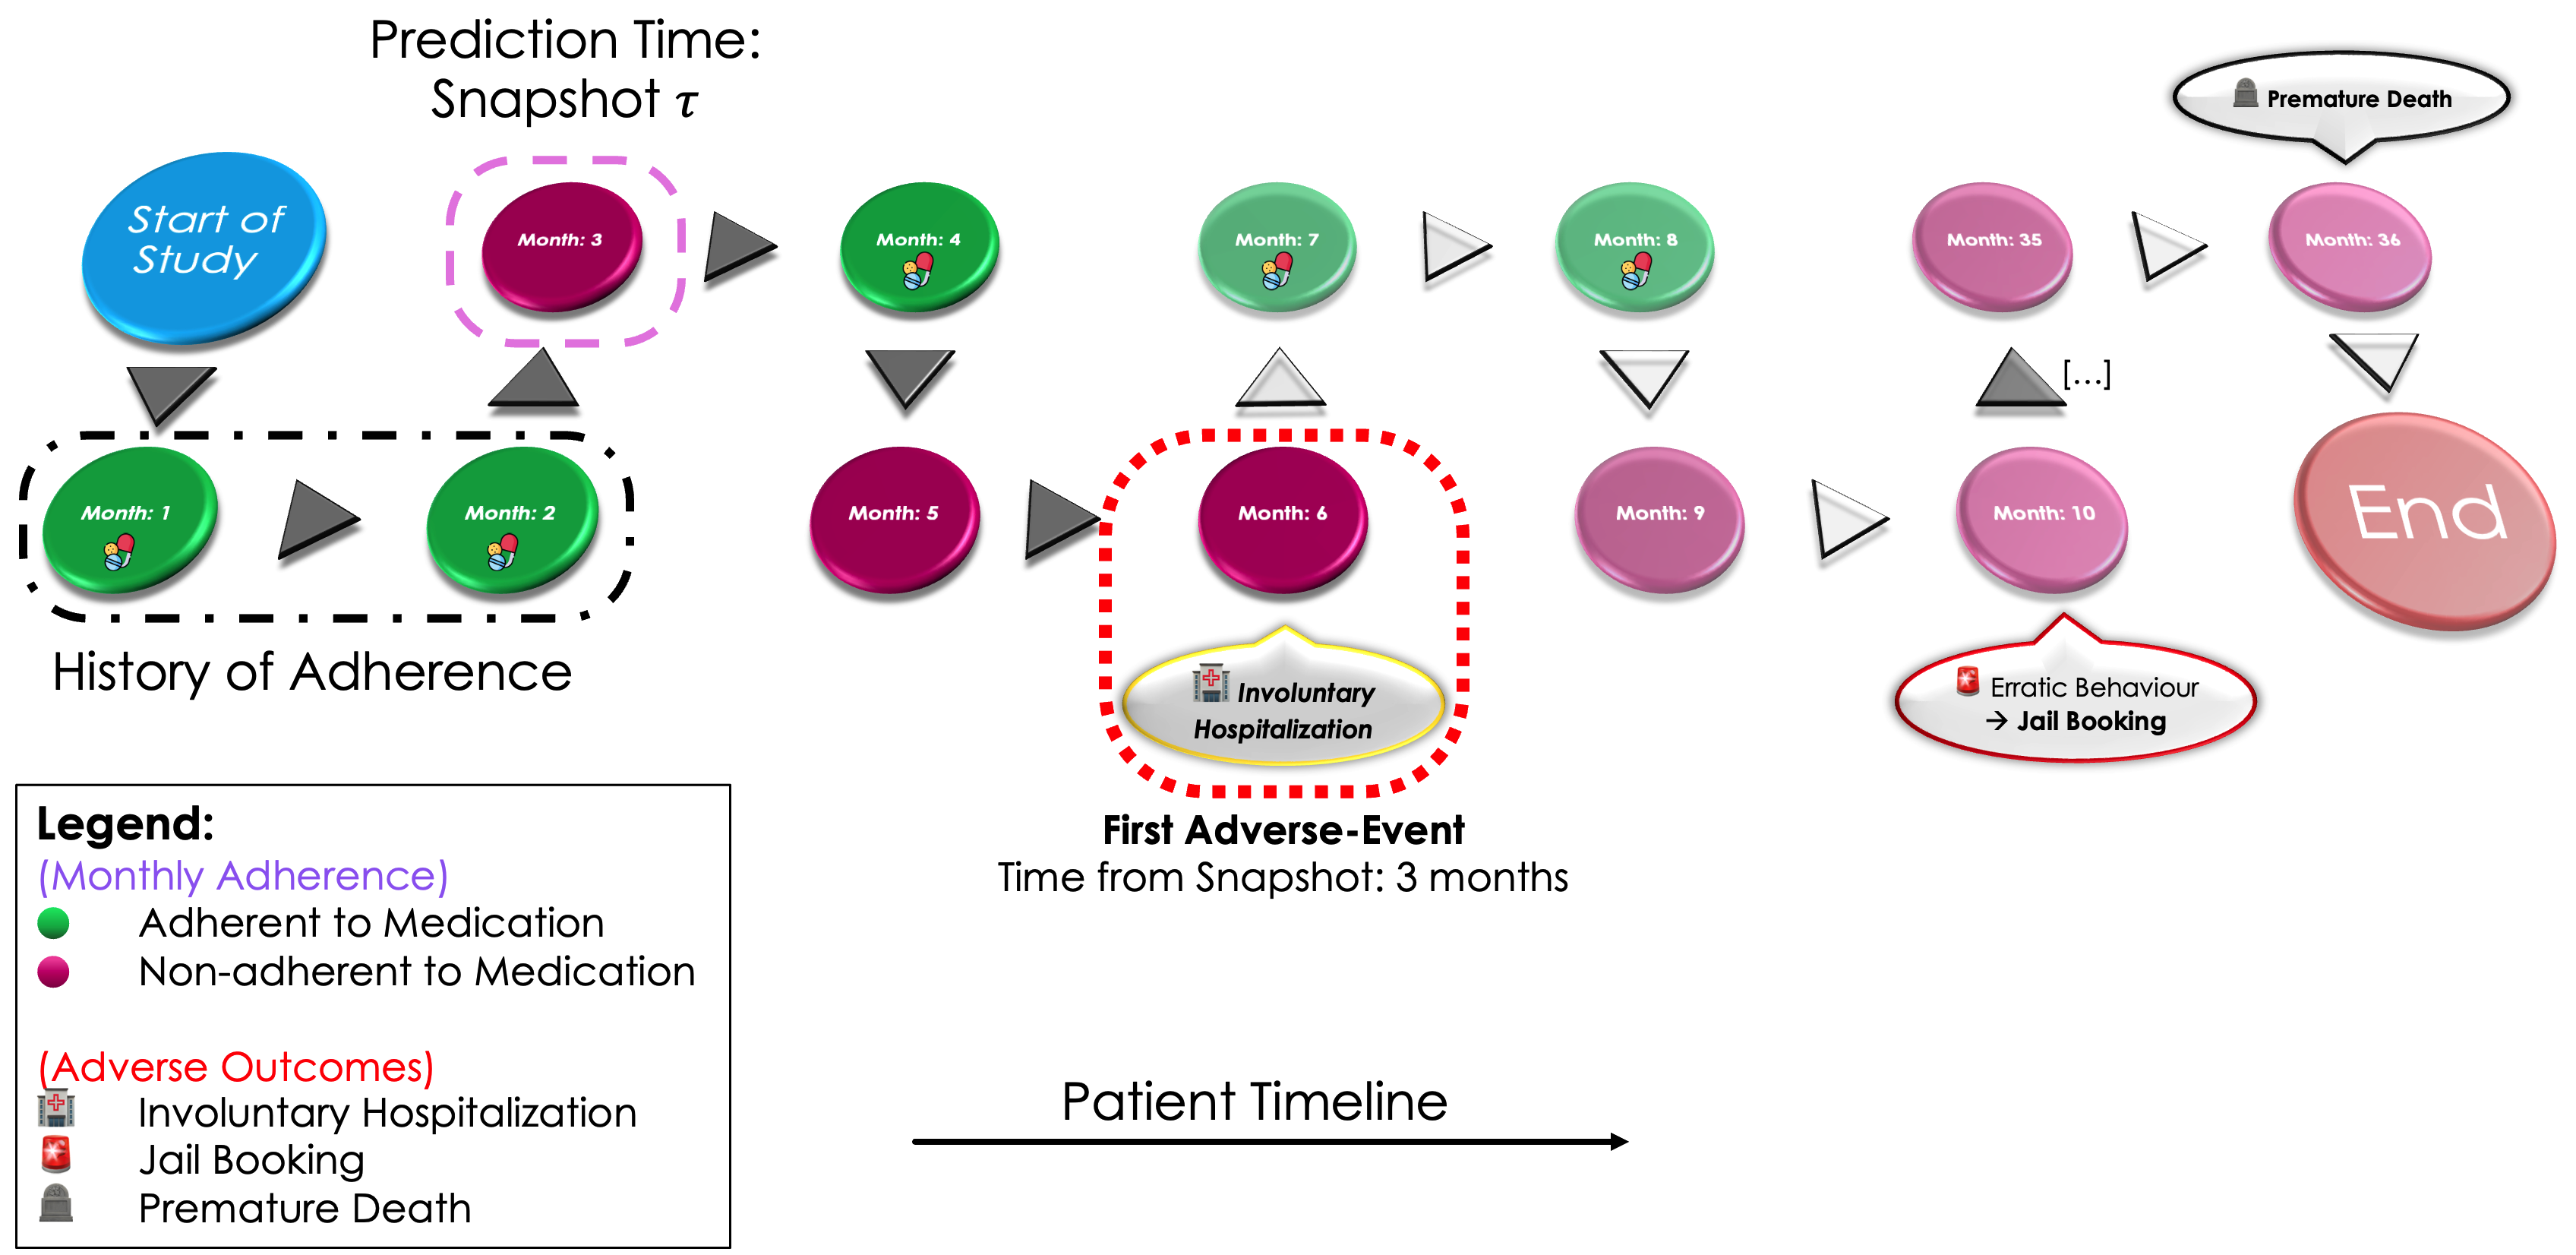
\includegraphics[width=.57\linewidth]{Figures/Overview/Causal_Survival_Analysis-Patient_Trajectory.png}}%
    \hspace{2.5em}
    \subfigure[Gender]{\label{fig:adherence_indicator}%
      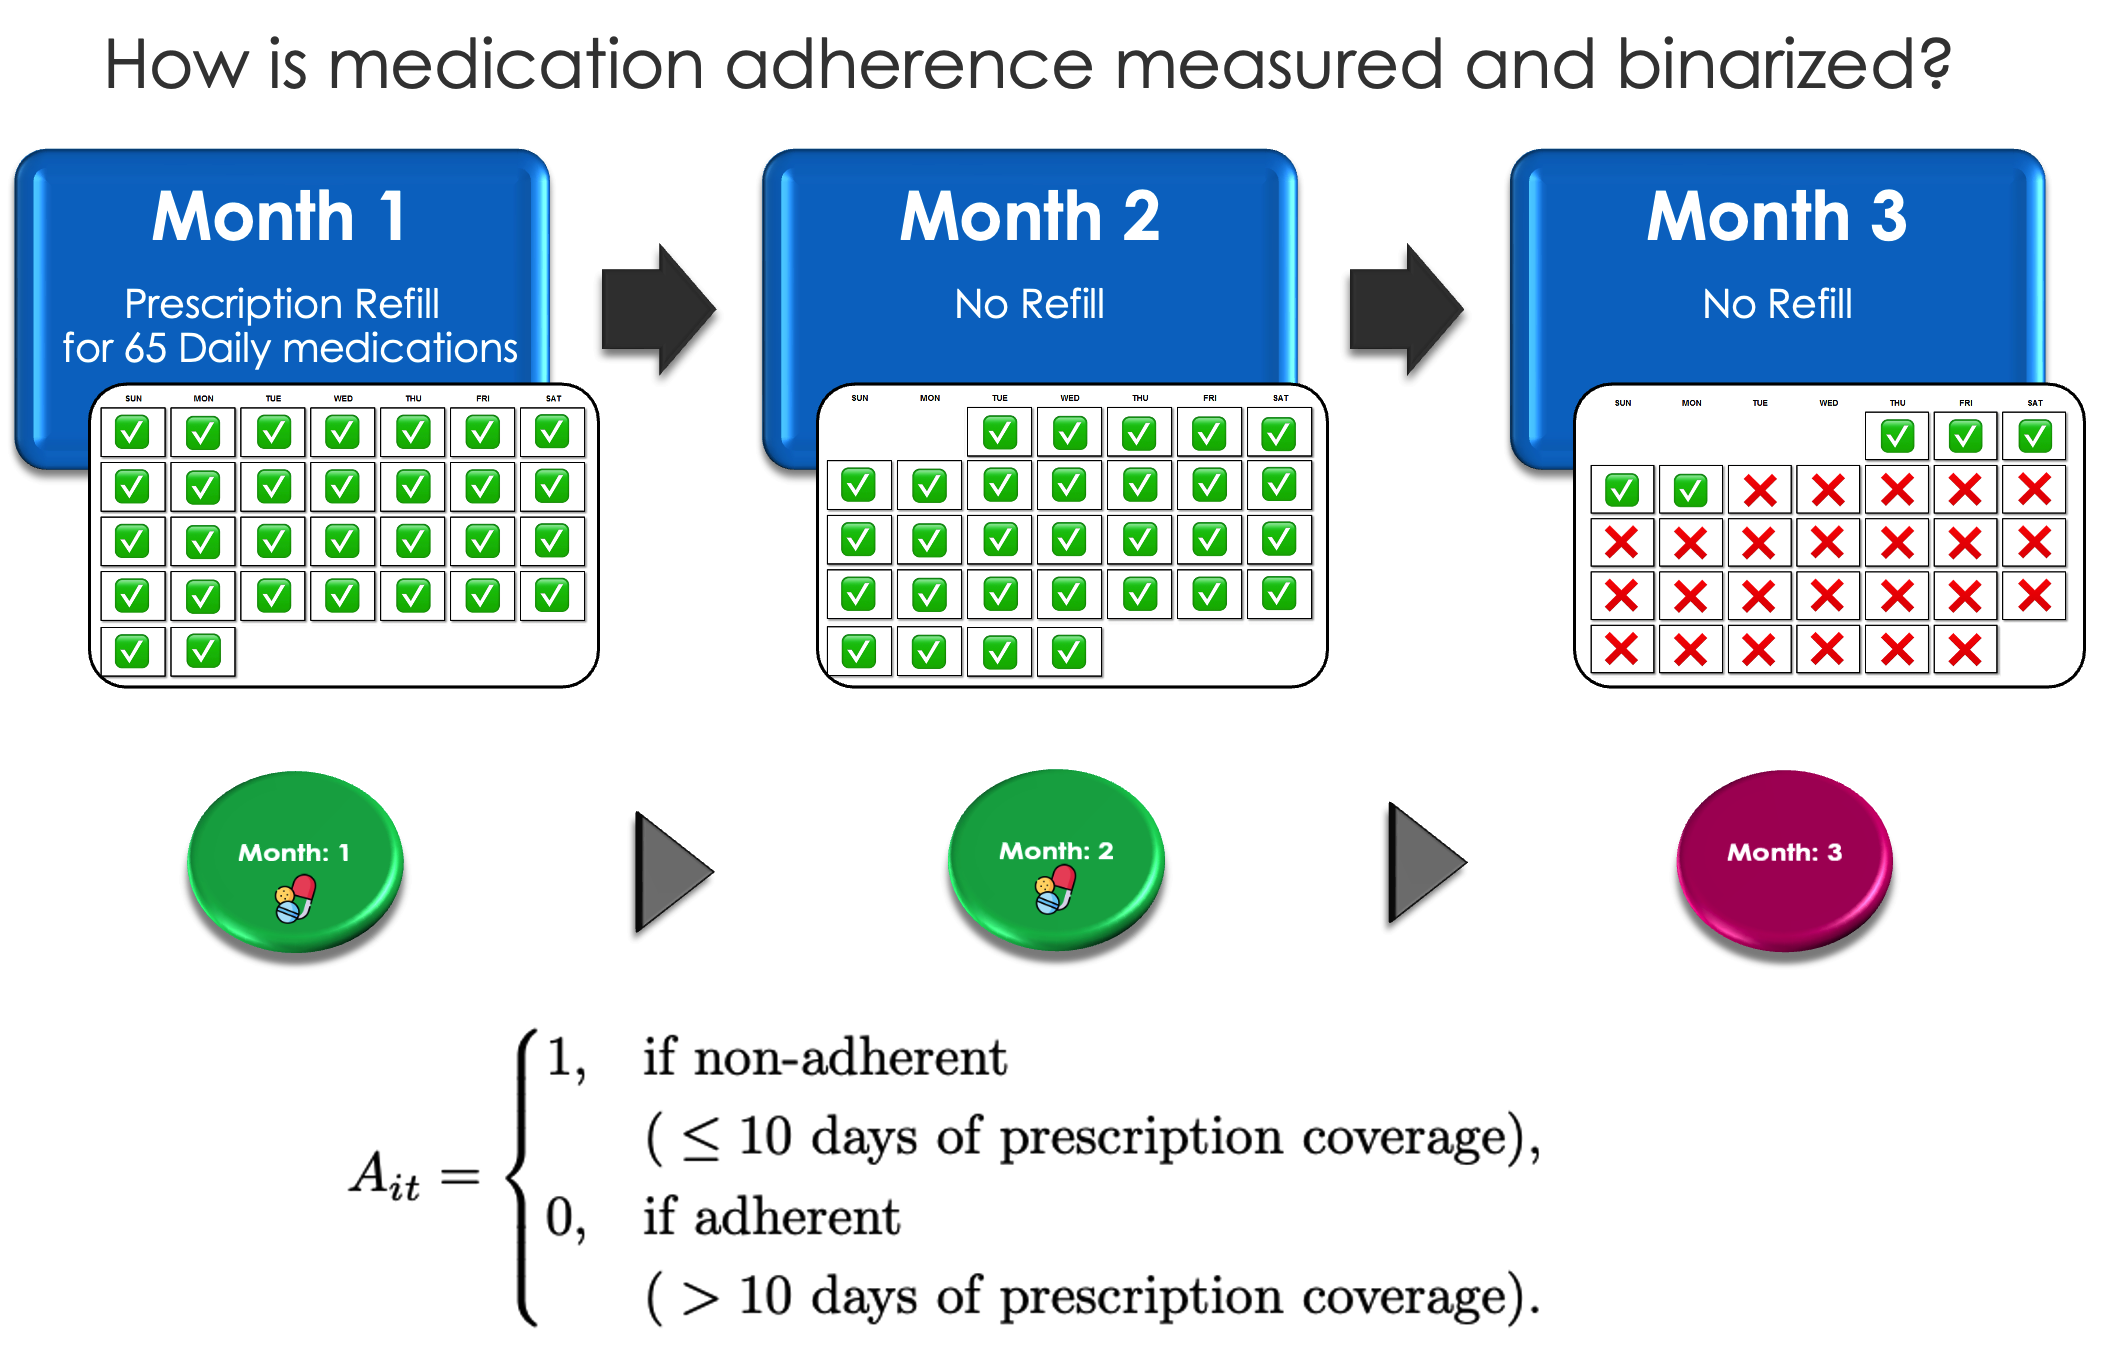
\includegraphics[width=.37\linewidth]{Figures/Overview/Causal_Survival_Analysis-Adherence_Level.png}}%
    }
\end{figure*}

The rest of this section provides a comprehensive overview of the study cohort, detailing its demographic composition, adverse event characteristics, adherence patterns, and prescribing trends for antipsychotic medications. 
This analysis aims to contextualize the characteristics of the patient population and identify key factors that may influence adherence behaviors. 
By examining static demographic covariates, the timing and type of adverse events, non-adherence trends, and medication-specific patterns, this section offers context for subsequent findings and their implications.

\subsubsection{Demographics}
\label{apd:cohort_demographics}

\begin{figure}[htbp]
\floatconts
  {fig:demographics}
  {\caption{Distribution of Static Demographic Covariates Across Patients in the Study Cohort.}}
  {%
    \subfigure[Age at the Beginning of the Study]{\label{fig:demographics_age}%
      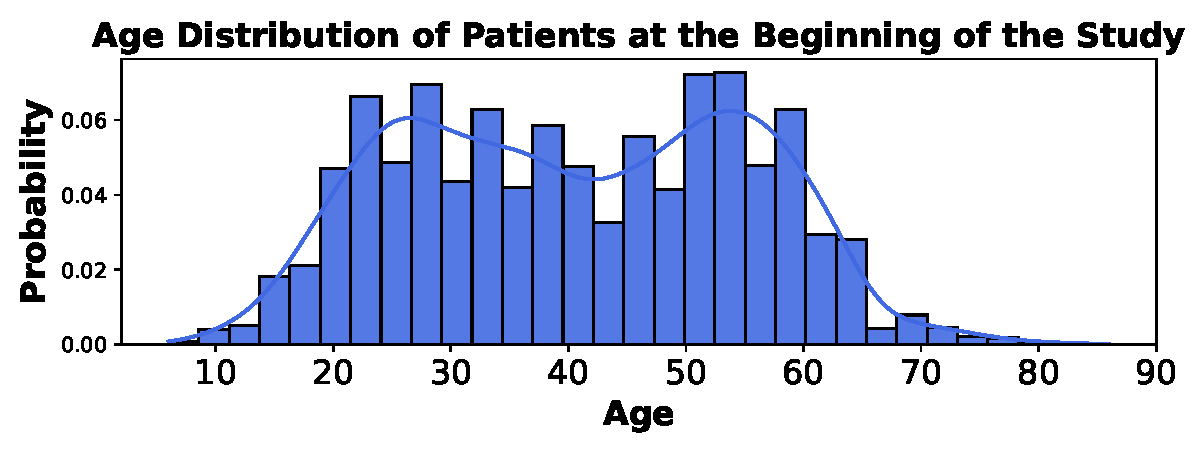
\includegraphics[width=.9\linewidth]{Figures/Demographics/age_distribution_at_beginning_of_study.pdf}}%
    \\
    \subfigure[Gender]{\label{fig:dempgraphics_gender}%
      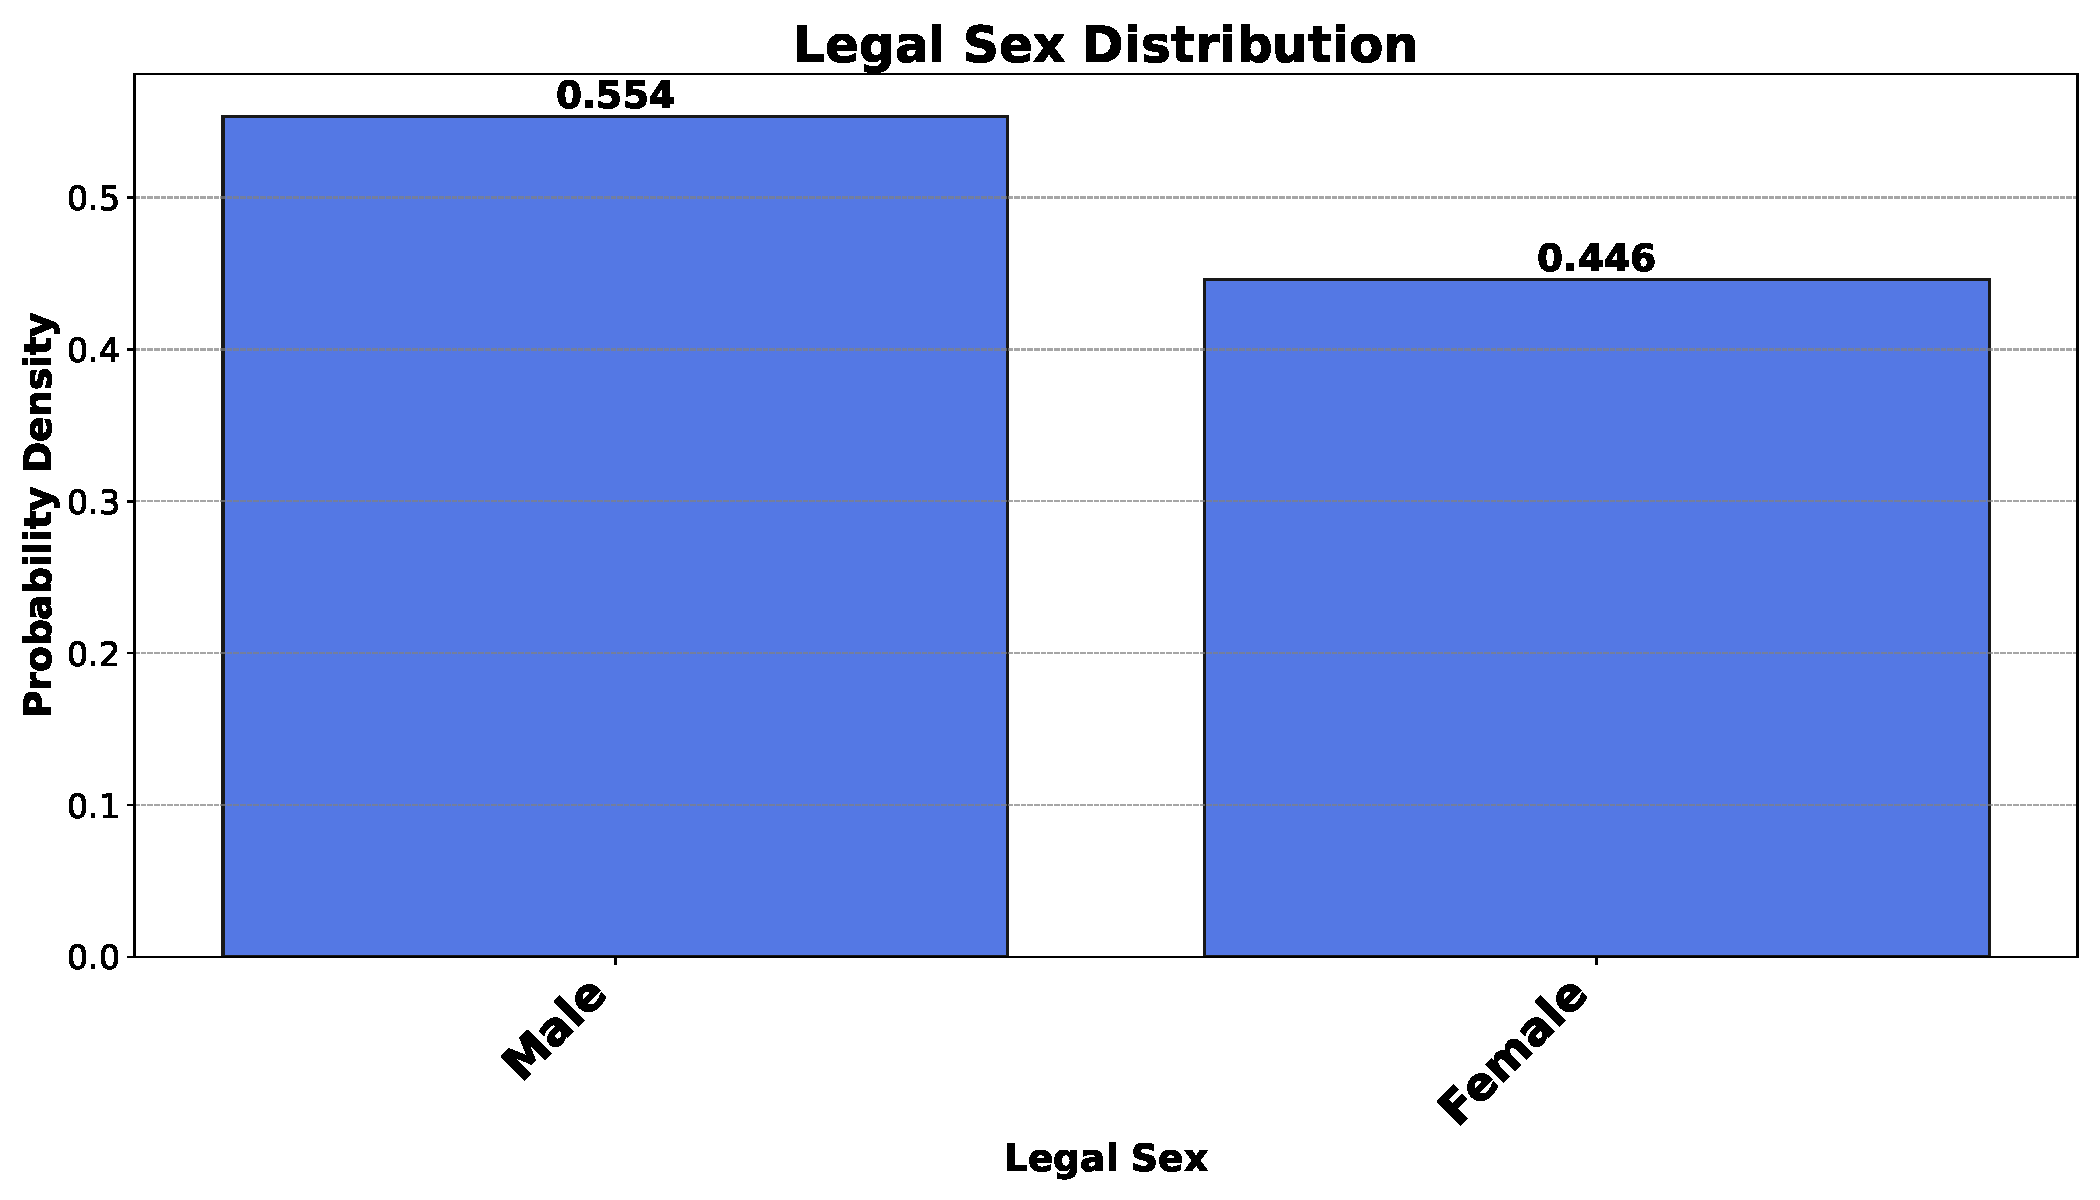
\includegraphics[width=.9\linewidth]{Figures/Demographics/distribution_of_legal_sex_among_patients.pdf}}%
    \\
    \subfigure[Race]{\label{fig:demographics_race}%
      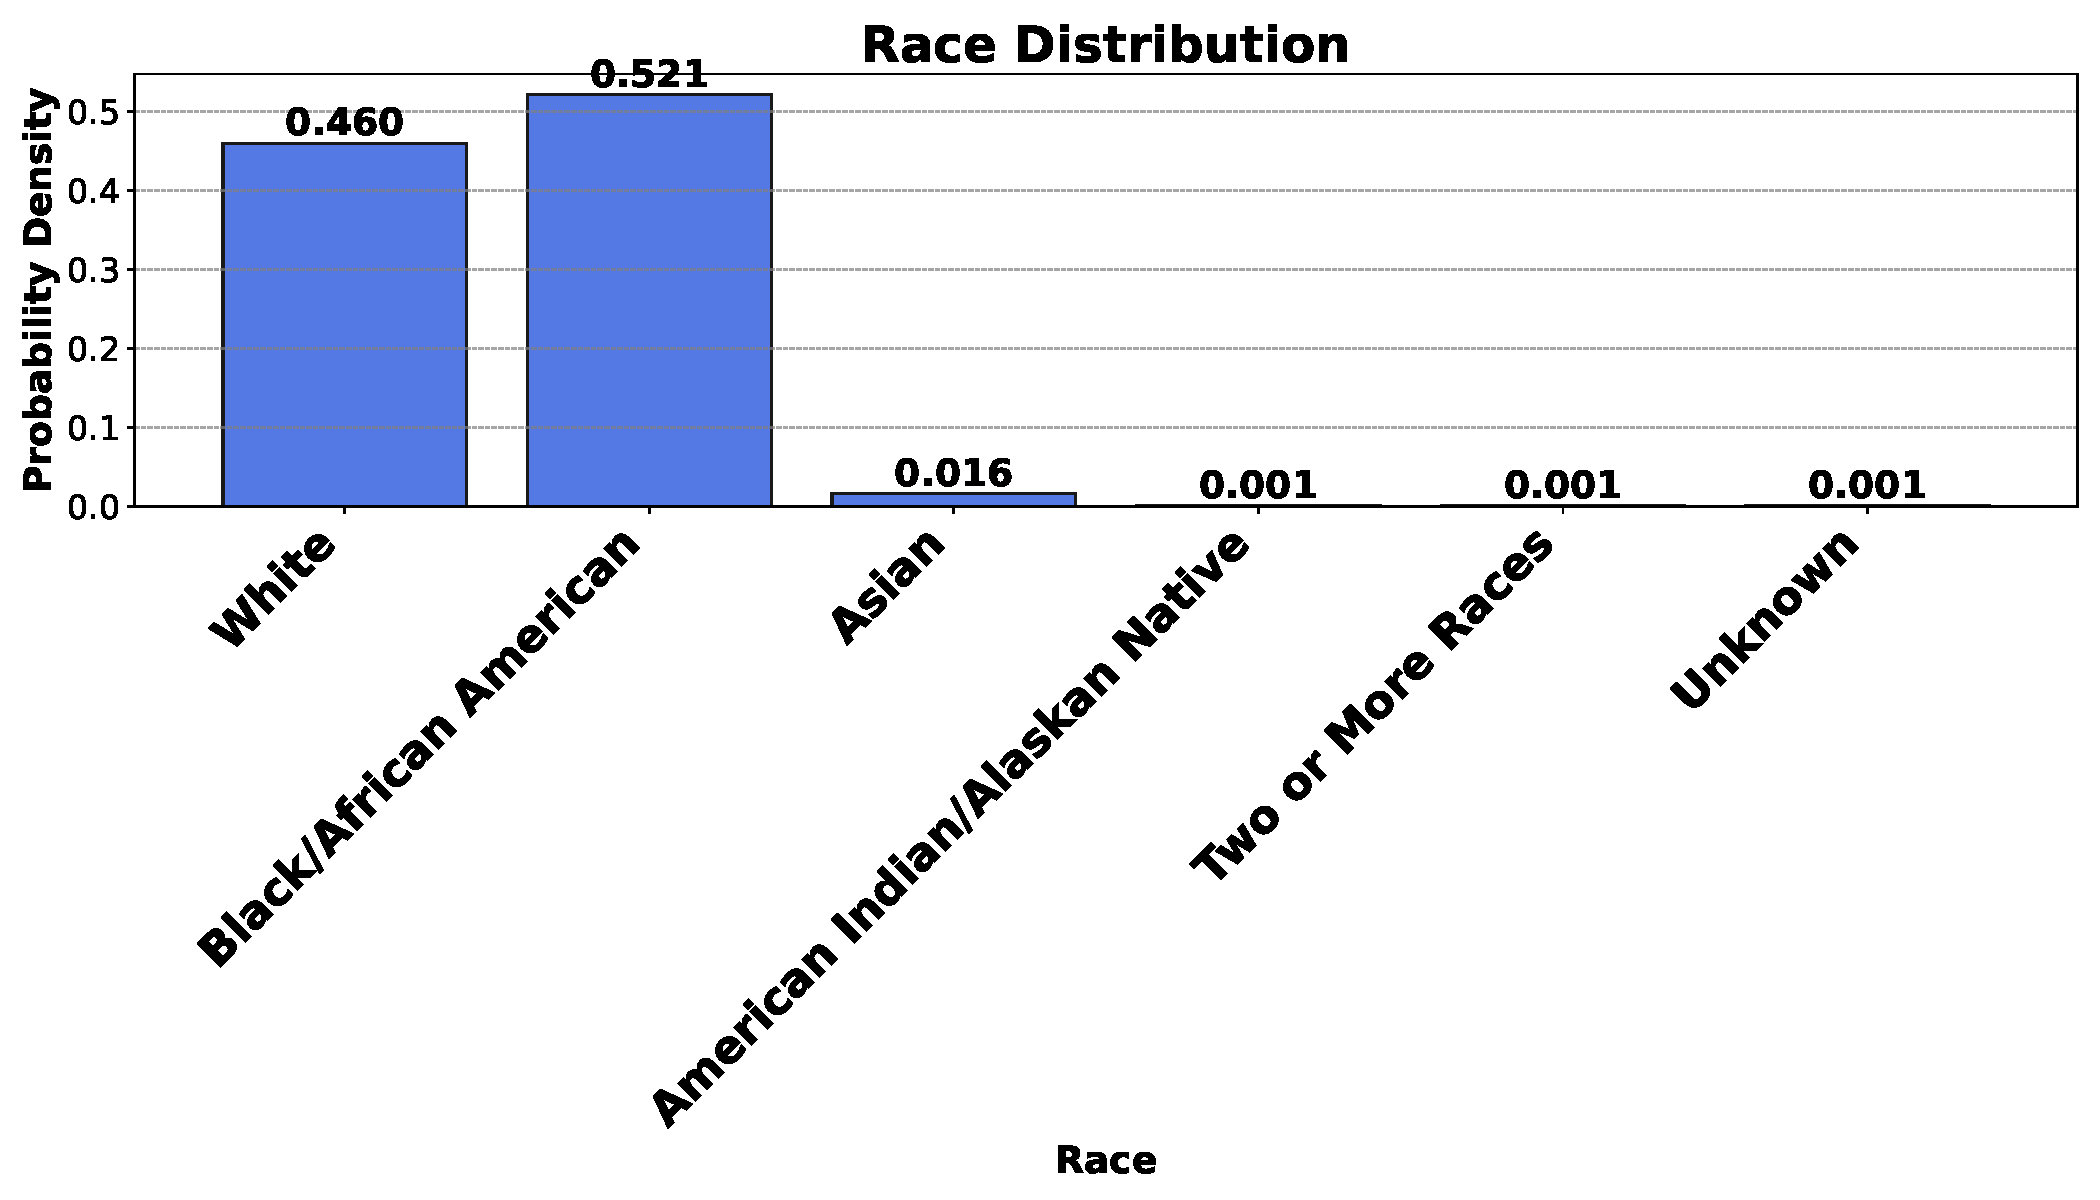
\includegraphics[width=.9\linewidth]{Figures/Demographics/distribution_of_race_among_patients.pdf}}%
    \\
    \subfigure[Education Level]{\label{fig:demographics_education}%
      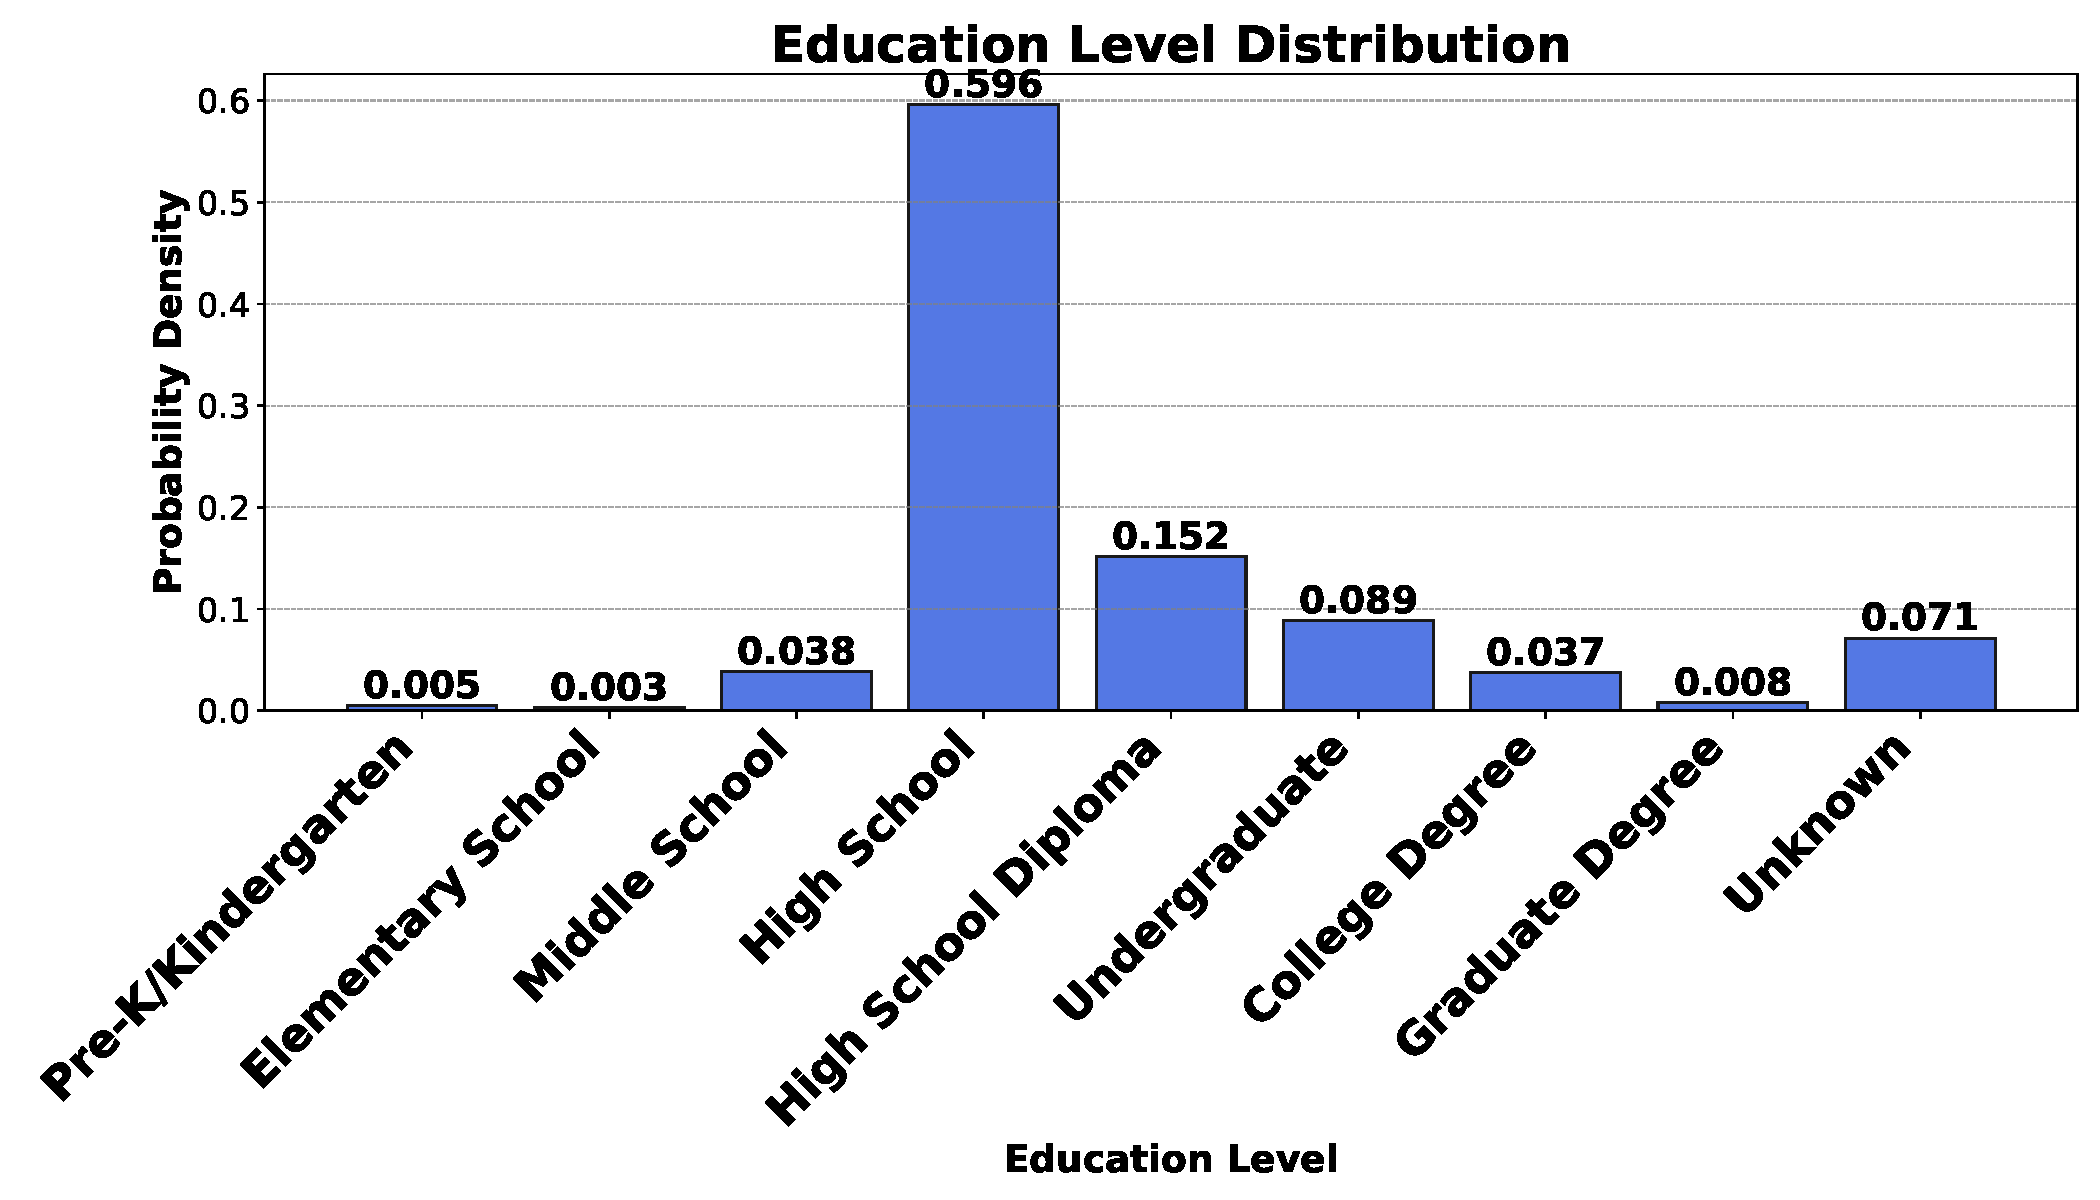
\includegraphics[width=.9\linewidth]{Figures/Demographics/distribution_of_education_level_among_patients.pdf}}%
  }
\end{figure}

The demographic characteristics of patients included in the study cohort are summarized in Figure~\ref{fig:demographics}.
 
Figure~\ref{fig:demographics_age} presents the age distribution of patients at the beginning of the study.
The cohort exhibits a broad age range, with the majority of patients aged between 30 and 60 years, and a peak density near 50 years.
This suggests that the study primarily captures middle-aged adults, though younger and older individuals are also represented.
 
The gender distribution is shown in Figure~\ref{fig:dempgraphics_gender}, with males comprising 55.4\% of the cohort and females making up 44.6\%.
This slight overrepresentation of males may reflect broader population trends or sampling biases in the study cohort.
 
Figure~\ref{fig:demographics_race} depicts the racial distribution of the cohort.
Black/African American patients form the largest racial group at 52.1\%, followed by White patients at 46.0\%.
Other racial groups, including Asian, American Indian/Alaskan Native, and multiracial individuals, are underrepresented, each contributing less than 2\% to the overall cohort.
 
The education level distribution, displayed in Figure~\ref{fig:demographics_education}, highlights that the majority of patients (59.6\%) have their education level at high school level.
A substantial proportion have high school diploma (15.2\%), while 8.9\% have enrolled in college.
The remaining patients have lower levels of formal education or their education status is unknown.

\subsubsection{First Adverse Event Type and Time}
\label{apd:cohort_first_event}

The timing and type of the first composite adverse event for patients in the study cohort are depicted in Figure~\ref{fig:first_event_time}. 
In the cohort of our study, the average time to a composite adverse event is 18.1 months. 
The average censoring time is 60.7 months.

Figure~\ref{fig:first_event_time_with_censoring} illustrates the distribution of the time to the first adverse event in months for all patients, including those who were right-censored. 
The histogram reveals that a substantial number of patients experience their first adverse event within the first 12 months of the study. 
The peak in adverse events at later months, specifically near the 96-month mark, coincides with patients who are censored at the end of the follow-up period. 

Figure~\ref{fig:first_event_time_without_censored_data} presents a similar distribution but excludes right-censored patients. 
The histogram demonstrates that the majority of adverse events occur within the first two years of the study, with a gradual decline in frequency over time. 
This decline reflects the decreasing number of at-risk patients as the study progresses. 

The distribution of event types for the first composite adverse event is summarized in Figures~\ref{fig:event_type_with_censoring} and \ref{fig:event_type_without_censored_data}. 
Figure~\ref{fig:event_type_with_censoring} includes all patients and highlights that over half of the cohort (54.3\%) were right-censored, with involuntary hospitalization comprising 24.4\% of events, followed by jail stays (13.2\%) and deaths (8.0\%). 

For patients who experienced an adverse event, Figure~\ref{fig:event_type_without_censored_data} shows that involuntary hospitalizations account for the majority (53.5\%), followed by jail stays (28.9\%) and deaths (17.6\%). 
The relative proportions of event types underscore the higher prevalence of involuntary hospitalization compared to other adverse events within the cohort of our study. 

\begin{figure*}[!htbp]
\floatconts
  {fig:first_event_time}
  {\caption{ (a)-(b) Distribution of Time of First Composite Adverse Event (in Months) across Patients Stacked by Each Adverse Event Type. 
  (a) includes patients with no adverse event (Right-Censored). 
  (b) presents the histogram of times only for patients with an adverse event recorded (Excluding Right-Censored Patients).
  (c)-(d) Distribution of Event Types within each Composite Adverse Event.}}
  {%
    \subfigure[All Patients]{\label{fig:first_event_time_with_censoring}%
      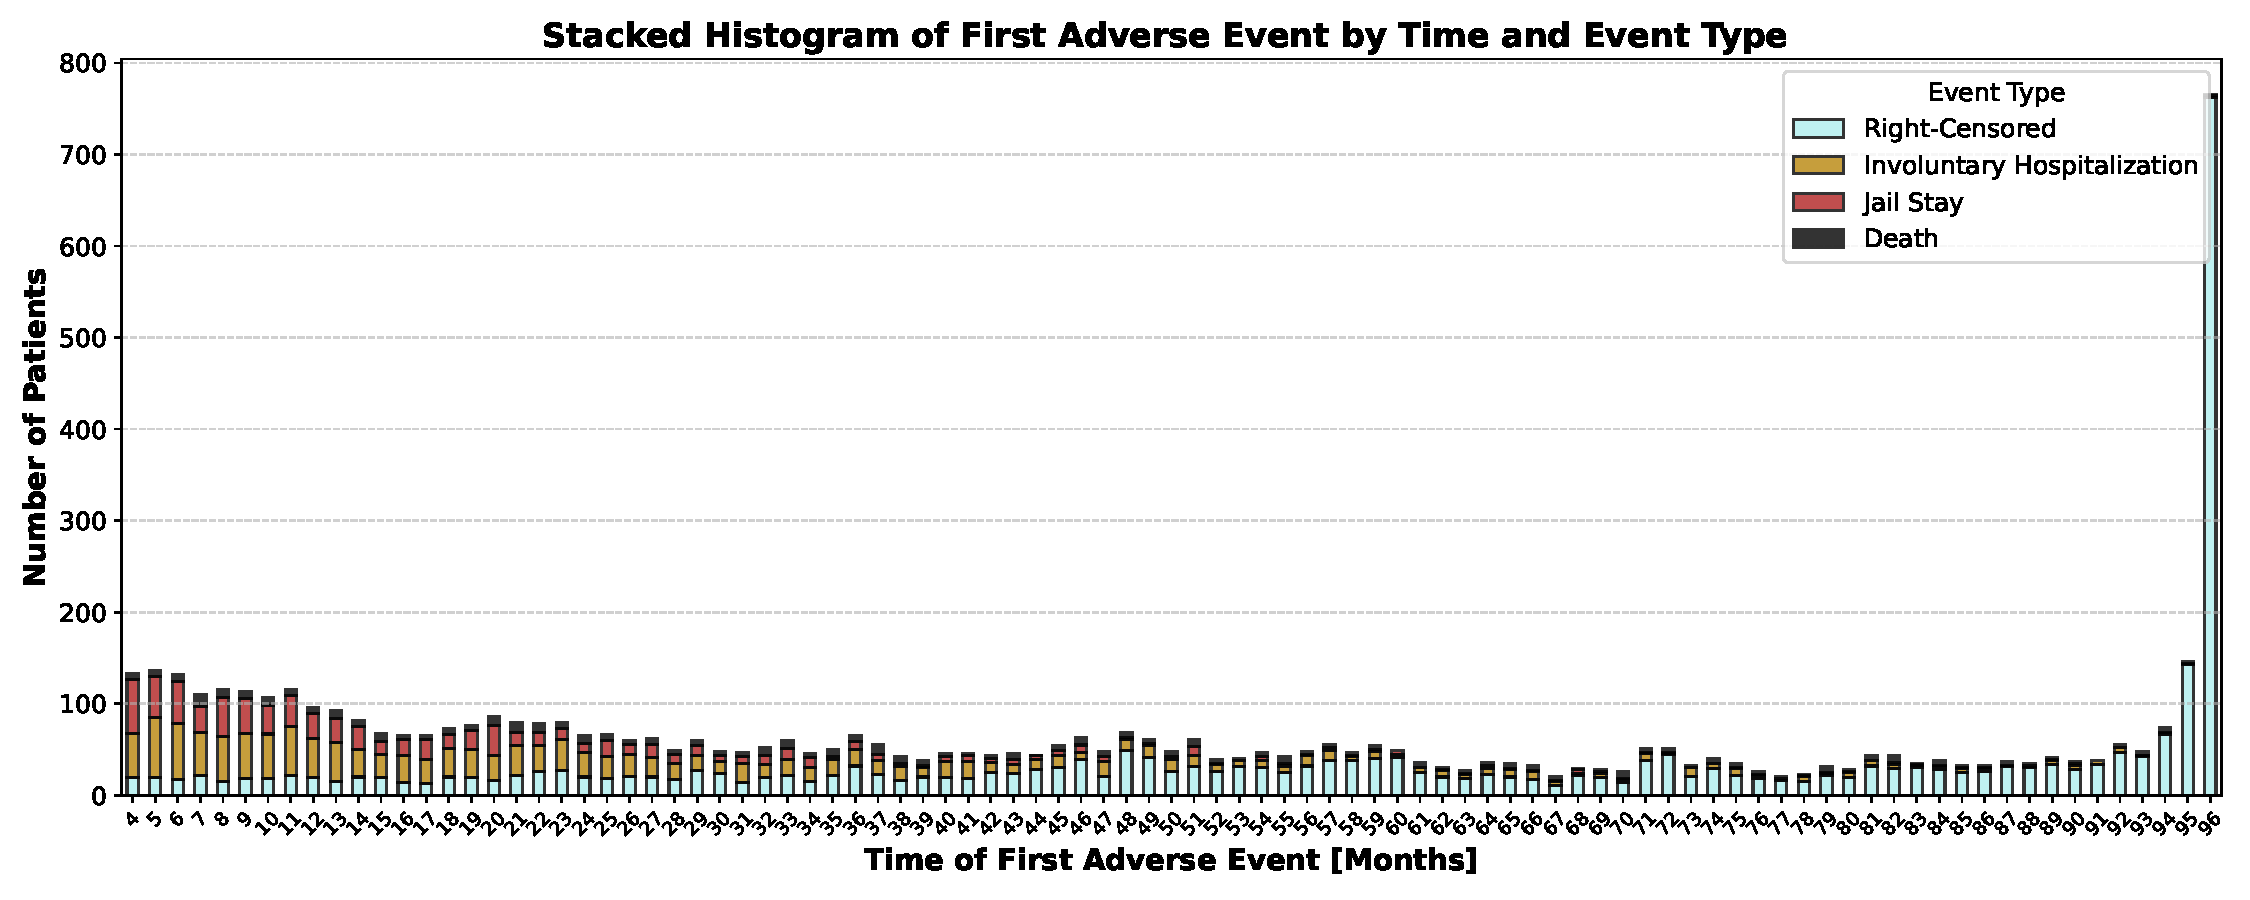
\includegraphics[width=0.9\linewidth]{Figures/First_Event/first_event_time_histogram.pdf}}%
    \\
    \subfigure[Patients with an Adverse Event]{\label{fig:first_event_time_without_censored_data}%
      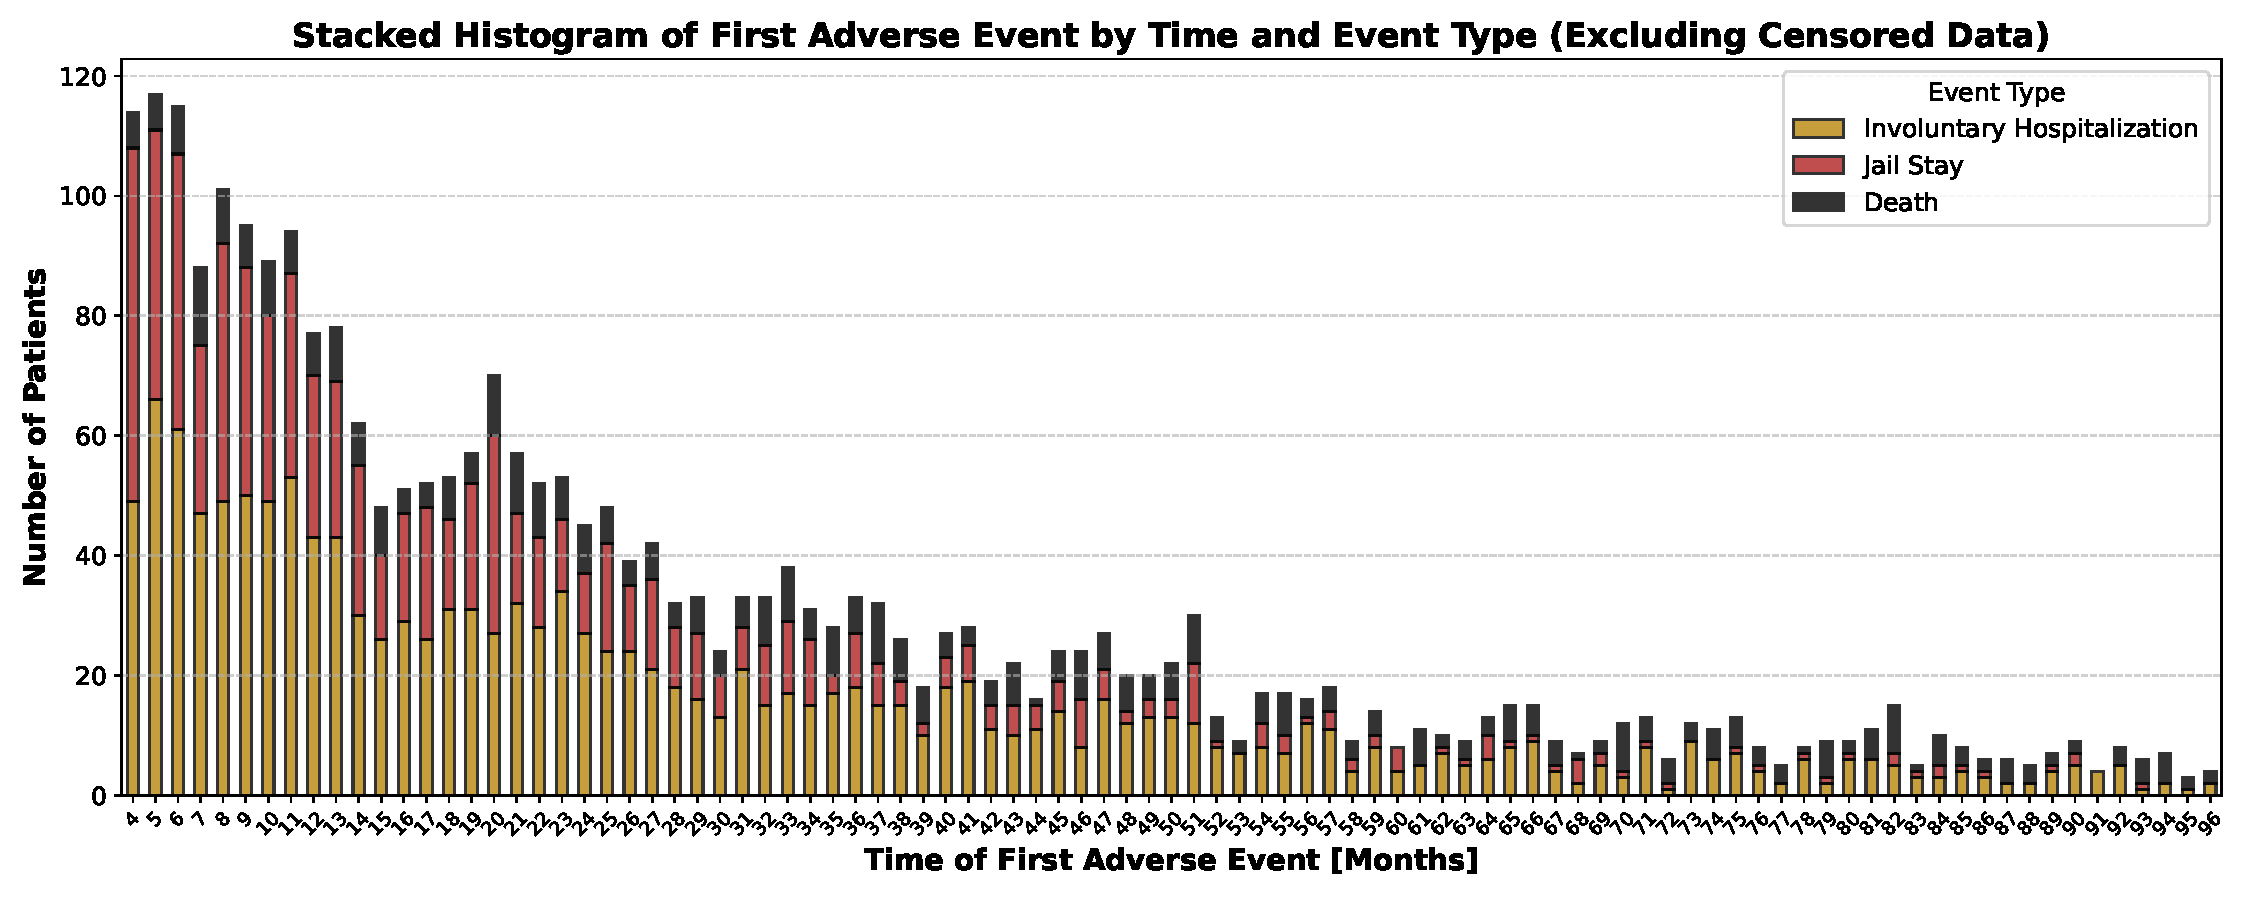
\includegraphics[width=0.9\linewidth]{Figures/First_Event/first_event_time_histogram_exclude_no_event.pdf}}%
    \\
    \subfigure[Event Type Distribution - All Patients]{\label{fig:event_type_with_censoring}%
      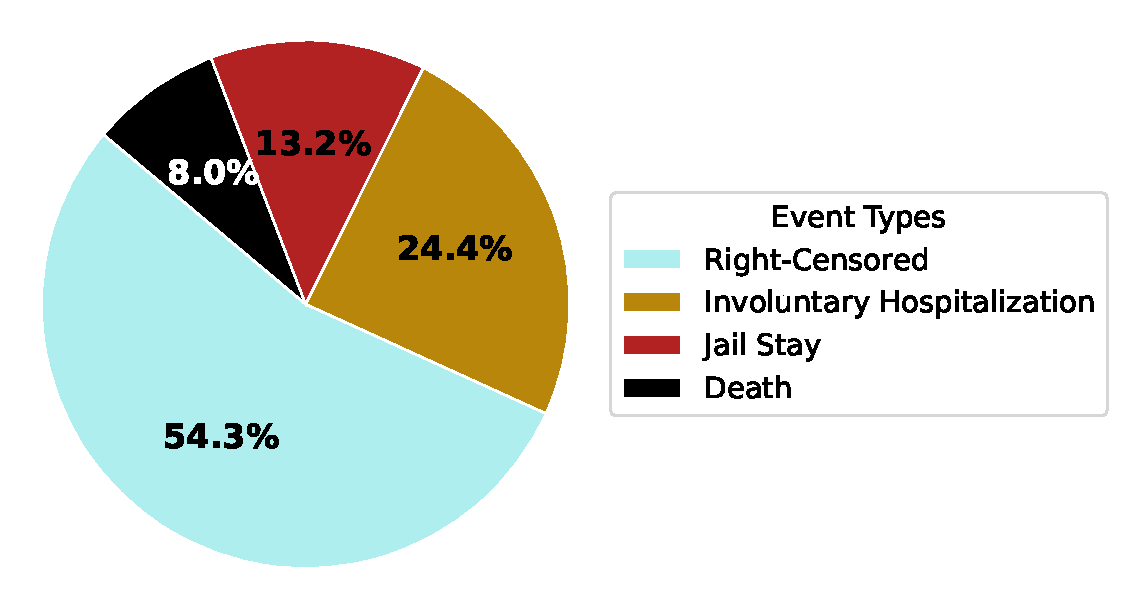
\includegraphics[width=0.4\linewidth]{Figures/First_Event/first_event_type_piechart.pdf}}%
    \qquad
    \subfigure[Event Type Distribution - Patients with an Adverse Event]{\label{fig:event_type_without_censored_data}%
      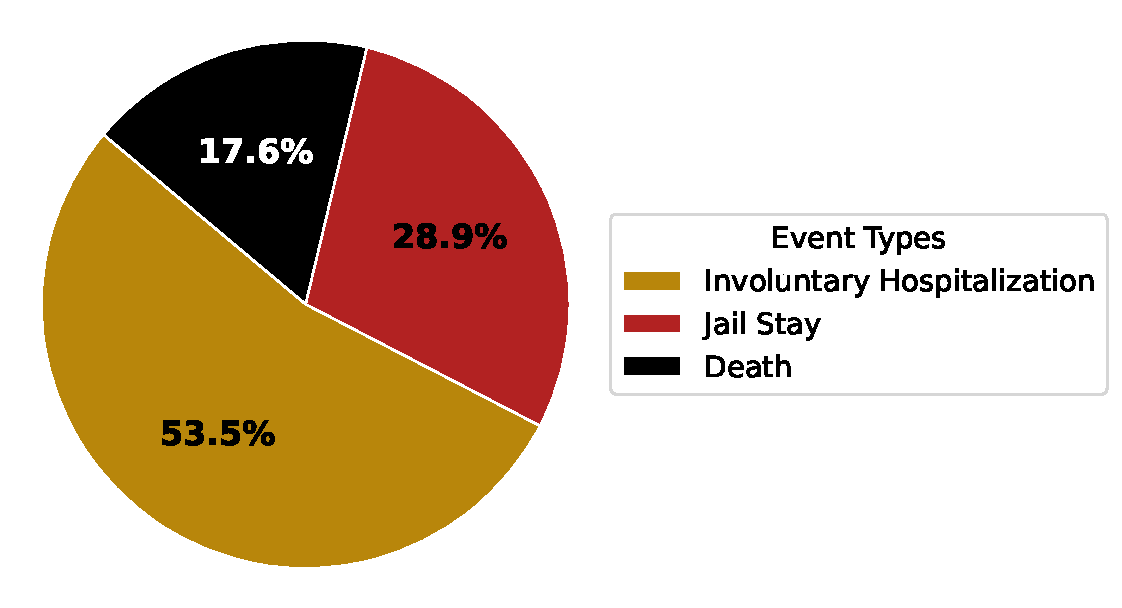
\includegraphics[width=0.4\linewidth]{Figures/First_Event/first_event_type_piechart_exclude_no_event.pdf}}%
  }
\end{figure*}

\subsubsection{Non-Adherence across Patients}
\label{apd:cohort_nonadherence}

Figure~\ref{fig:non_adherence_level} presents the distribution of average continuous non-adherence across patients in the cohort, highlighting differences in adherence patterns based on medication administration.

In Figure~\ref{fig:non_adherence_all}, the histogram illustrates non-adherence across all patients, with a bimodal distribution.
A significant proportion of patients are on average fully adherent, averaging zero days of non-adherence per month.
Conversely, another cluster of patients demonstrates complete non-adherence, averaging nearly 30 days of non-adherence per month.
As per the approach taken in Section~\ref{sec:methods_data}, we use a binary treatment indicator in our study for non-adherence. 
Patients with less than 10 days of non-coverage in a month are considered to be adherent to their medication in that month and subsequently non-adherent if they have more than 10 days of non-coverage in that month (represented in blue and red bars respectively in Figure~\ref{fig:non_adherence_level}).

Figure~\ref{fig:non_adherence_injectable} focuses on patients prescribed injectable medications at least once in their trajectory.
These patients exhibit more balanced adherence patterns compared to the overall cohort, with fewer patients at the extremes of complete non-adherence and relatively the same proportion of patients show full adherence on average in their month as the complete cohort.
It should be noted that if a patient is administered with an injectable in a month, they cannot be fully non-adhered in that month (hence there is no bar at day 30).

In contrast, Subfigure~\ref{fig:non_adherence_non_injectable} examines patients prescribed only non-injectable medications.
This group shows a higher tendency toward complete non-adherence, with a more pronounced peak near 30 days of non-adherence. 
The complete adherence pattern however is similar to that of the full cohort with 8\% of patients showing complete adherence to their prescribed drugs.

The comparison between subgroups suggests that the type of prescribed medication plays a role in influencing adherence behavior.
Injectable medications may be associated with better adherence due to their administration requirements and monitoring, while non-injectable medications exhibit greater variability in patient adherence patterns.
However, in our cohort only 26\% of patients were ever administered an injectable medication throughout the time they were involved in this study.
For this reason, in future work, it is equally important to focus on interventions and strategies that address adherence challenges specific to patients prescribed non-injectable medications, as they constitute the majority of the cohort.


\begin{figure}[htbp]
\floatconts
  {fig:non_adherence_level}
  {\caption{Distribution of Average Continuous Non-Adherence across Patients. (a) All Patients, (b) Patients prescribed with Injectable Medications (at least once in their trajectory), (c) Patients prescribed with Non-Injectable Medications. The x-axis shows the number of days in a month that a patient goes non-adherent on average. Non-coverage of less than 10 days in month is considered \textcolor{blue}{Adherent}, and for more than 10 days is considered \textcolor{red}{Non-Adherent} in our setup.}}
  {%
    \subfigure[All Patients]{\label{fig:non_adherence_all}%
      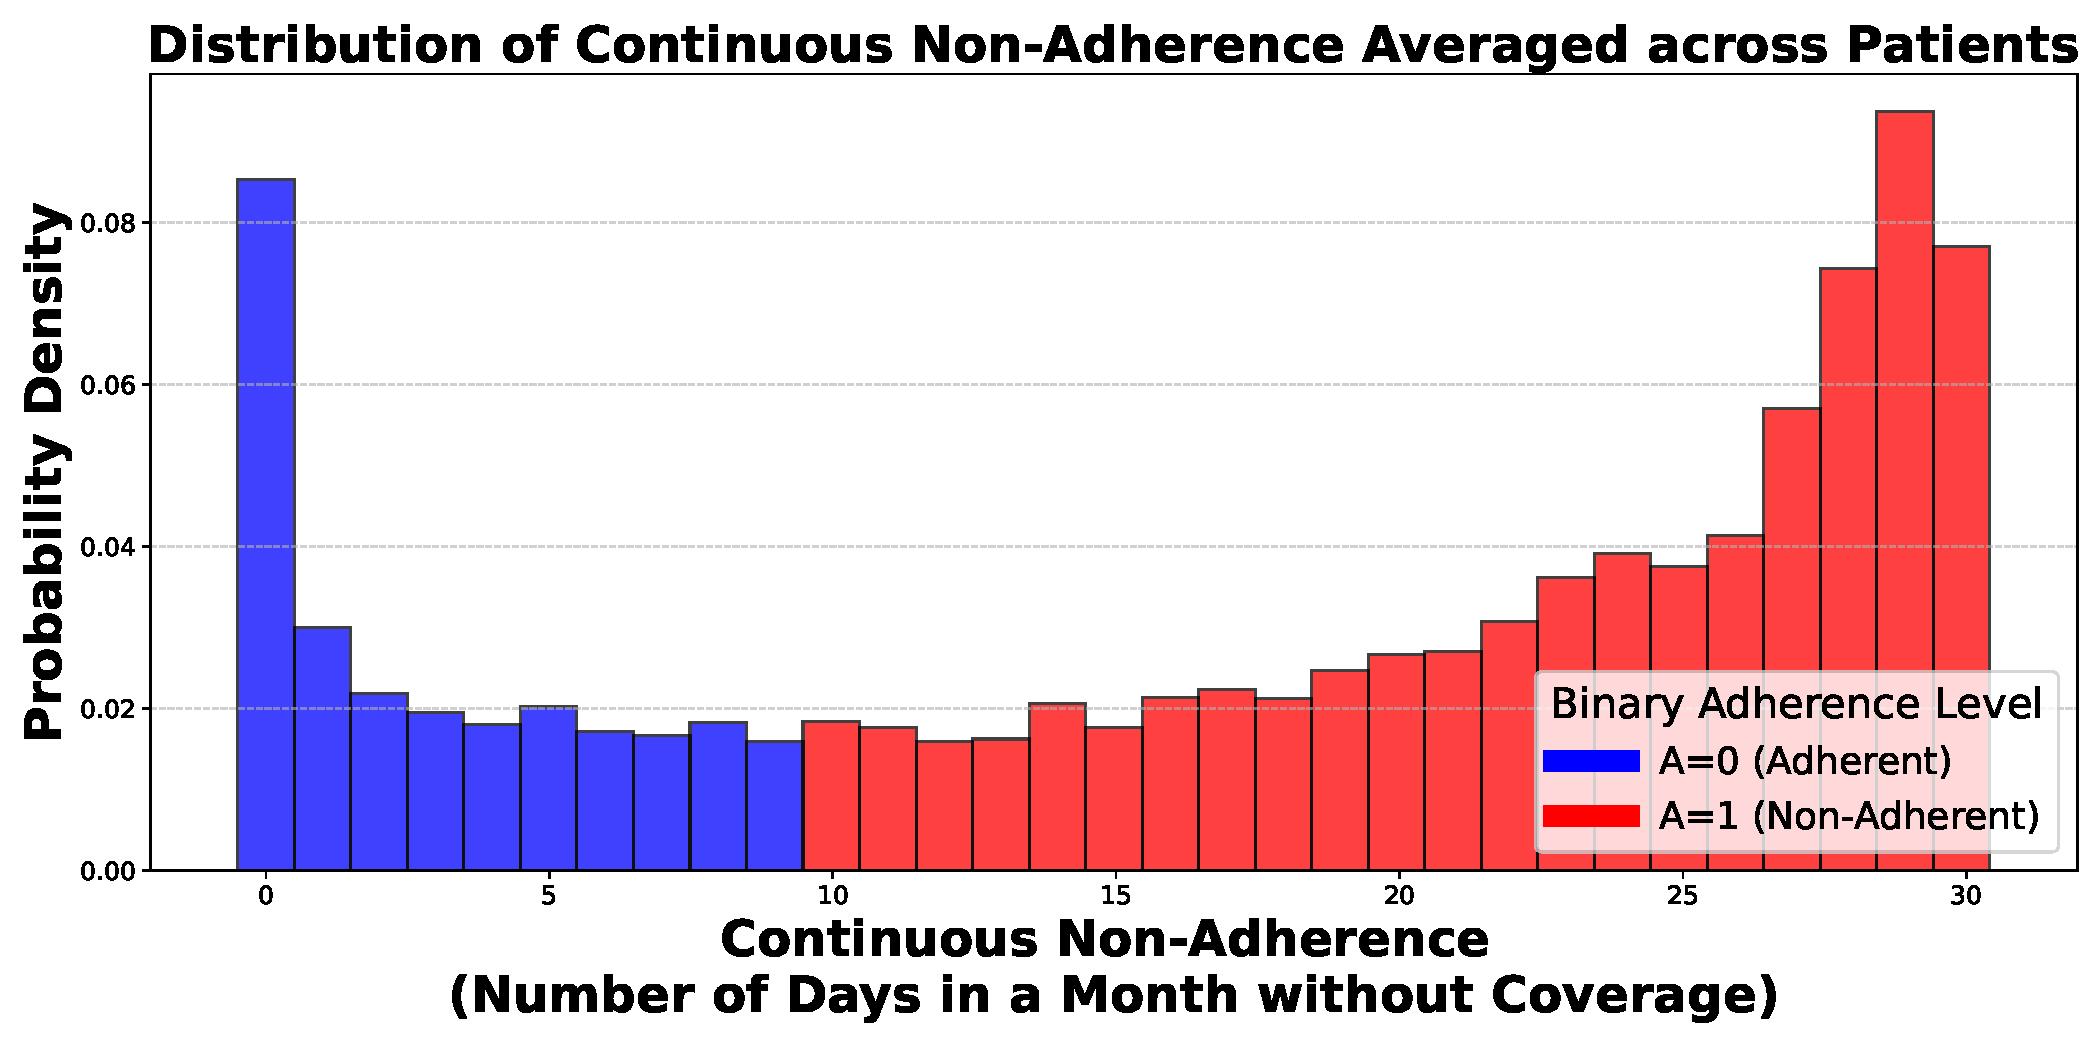
\includegraphics[width=\linewidth]{Figures/Non_Adherence_Levels/distribution_of_continuous_non-adherence_for_all_patients.pdf}}%
    \\
    \subfigure[Patients with Injectable Medication]{\label{fig:non_adherence_injectable}%
      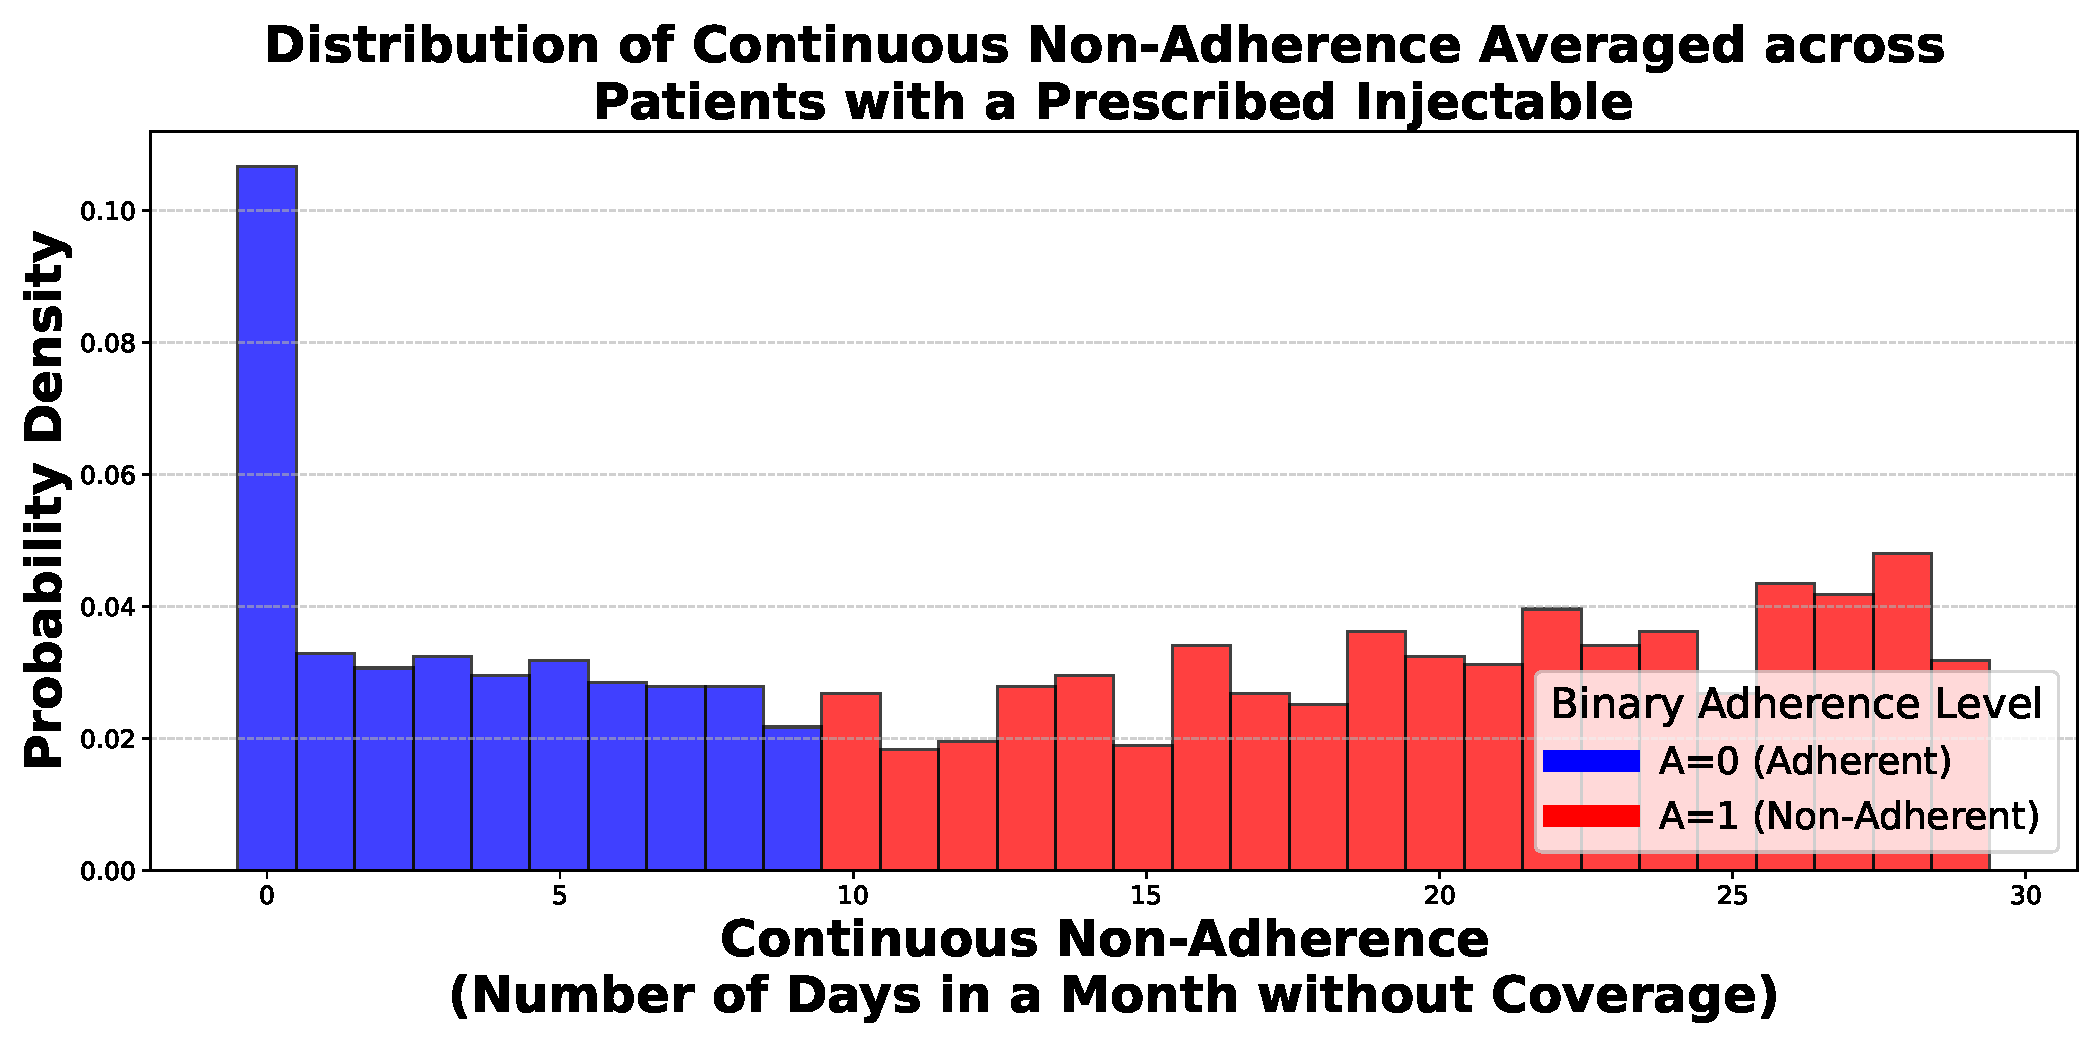
\includegraphics[width=\linewidth]{Figures/Non_Adherence_Levels/distribution_of_continuous_non_adherence_for_patients_with_injectables.pdf}}%
    \\
    \subfigure[Patients with Non-Injectable Medication]{\label{fig:non_adherence_non_injectable}%
      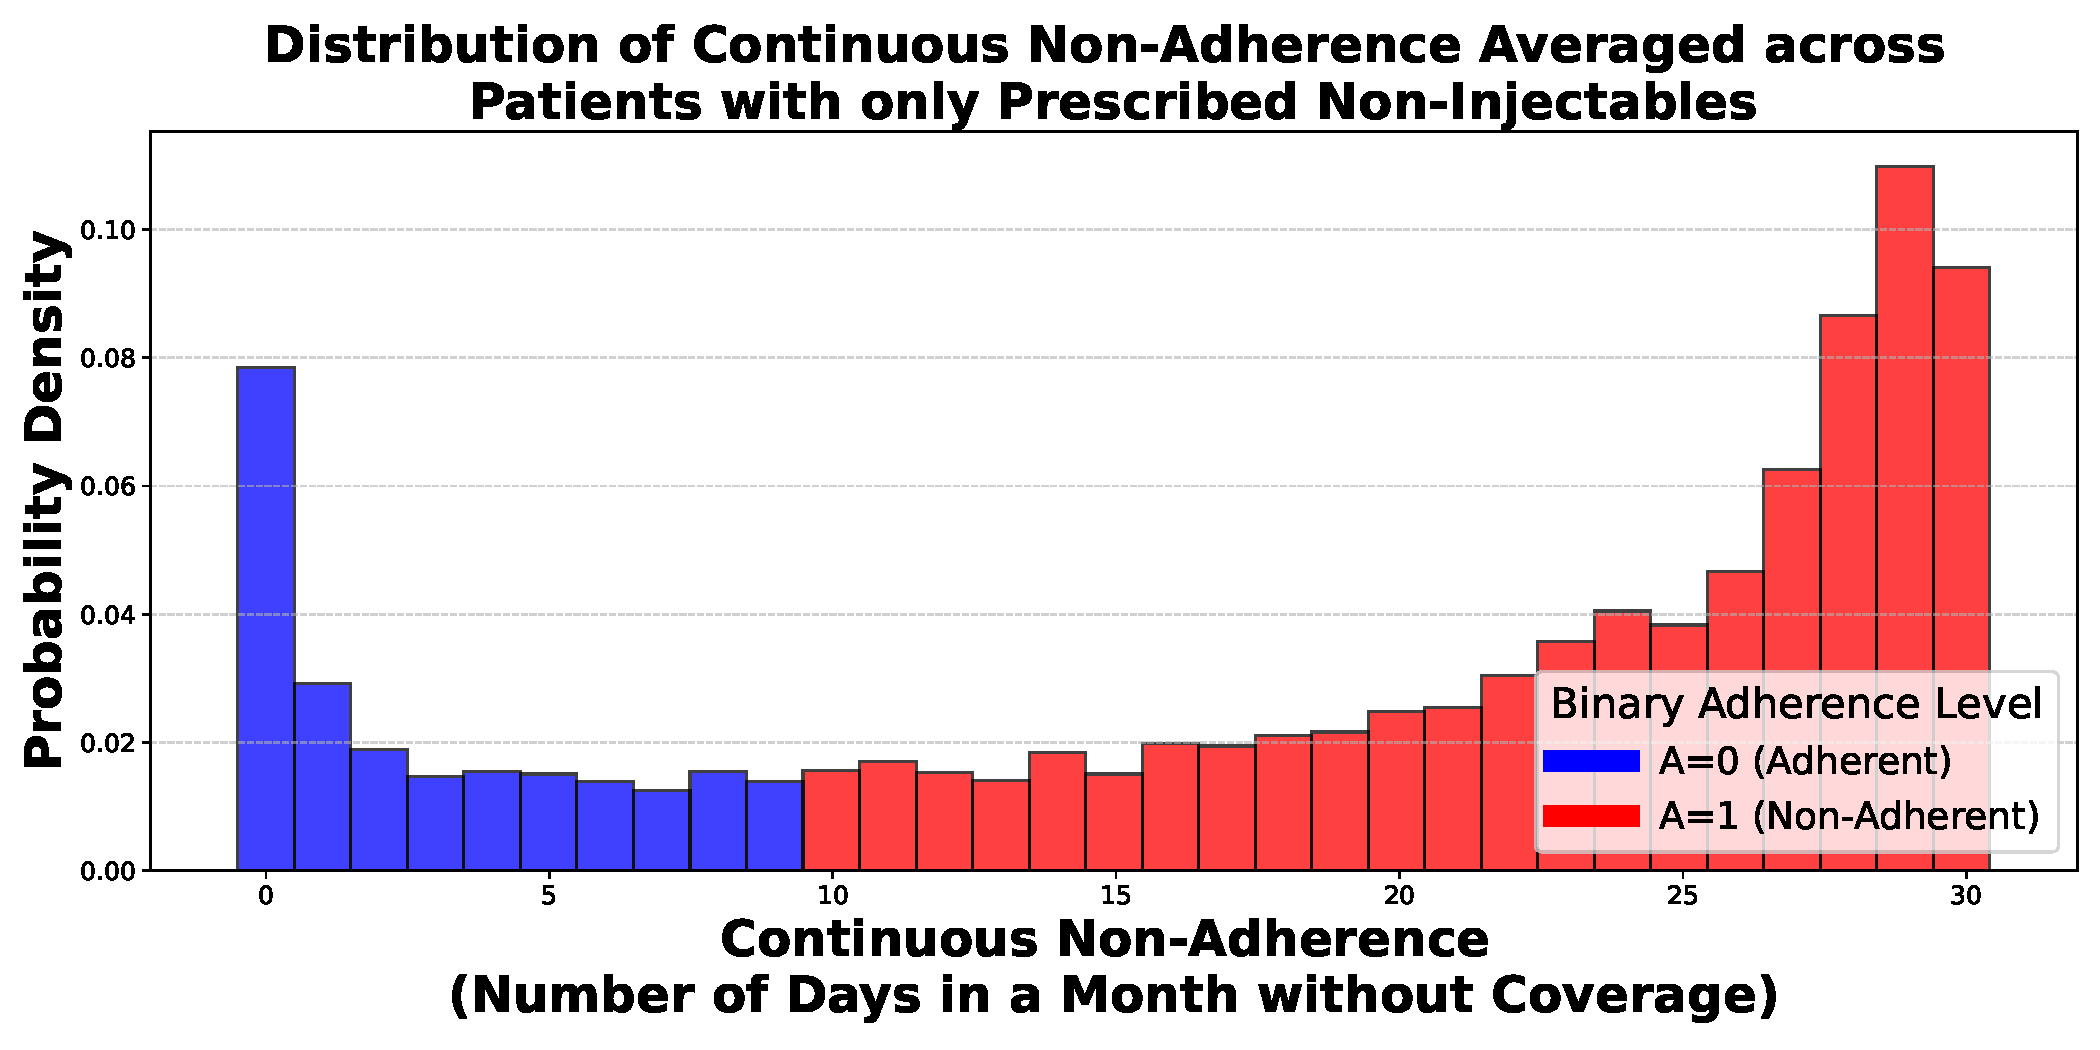
\includegraphics[width=\linewidth]{Figures/Non_Adherence_Levels/distribution_of_continuous_non_adherence_for_patients_with_non-injectables.pdf}}%
  }
\end{figure}

\subsubsection{Antipsychotic Medications}
\label{adp:cohort_medications}

\begin{figure*}[htbp]
\floatconts
  {fig:medications}
  {\caption{Prevalence of Antipsychotic Medications in the Patient Cohort. (a) Illustrates the percentage of patients prescribed each antipsychotic medication within the study cohort. The x-axis lists the medication names, and the y-axis represents the proportion of patients, expressed as a percentage. This visualization highlights the most frequently prescribed antipsychotic medications, with risperidone, aripiprazole, and olanzapine being the most prevalent. 
  (b), (c), and (d) Show the demographic composition of patients using each medication for (b) Legal Sex, (c) Race (c), and (d) Education Level. 
  (e) Shows the average age of patients using each antipsychotic medication.
  (f) Presents the mean continuous non-adherence scores for each antipsychotic medication. The y-axis values can range between 0 and 1 where a score of 1 indicates complete non-adherence, and a score of 0 represents full adherence.
}}
  {%
    \subfigure[Antipsychotic Medications Prevalence]{\label{fig:medication_prevalence}%
      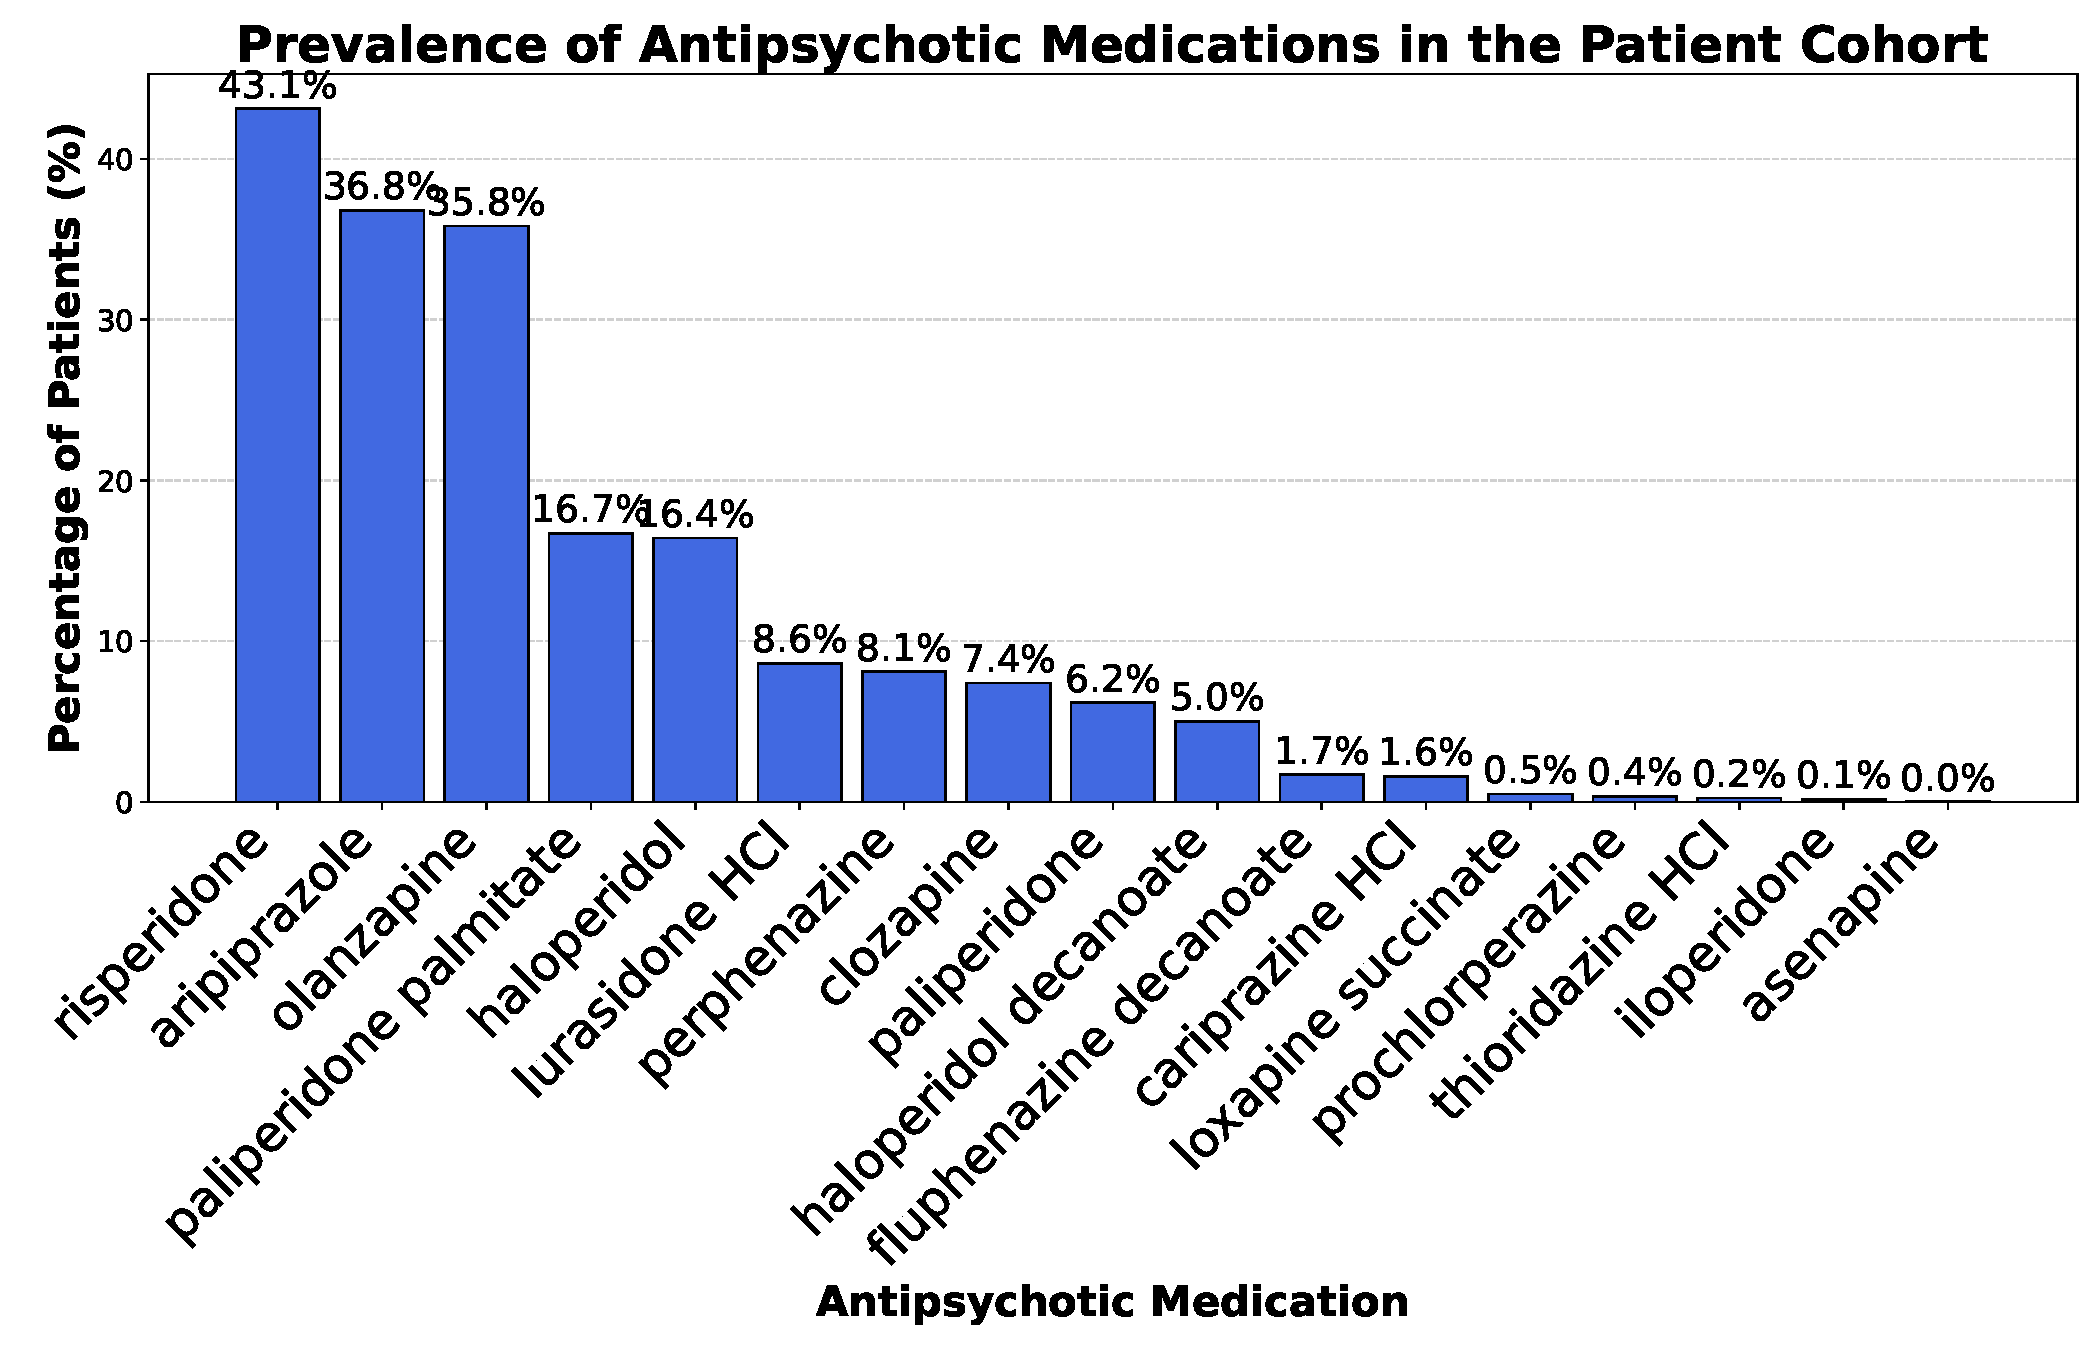
\includegraphics[width=0.458\linewidth]{Figures/Medications/antipsychotic_medication_prevalence.pdf}}%
    \qquad
    \subfigure[Gender]{\label{fig:medication_gender}%
      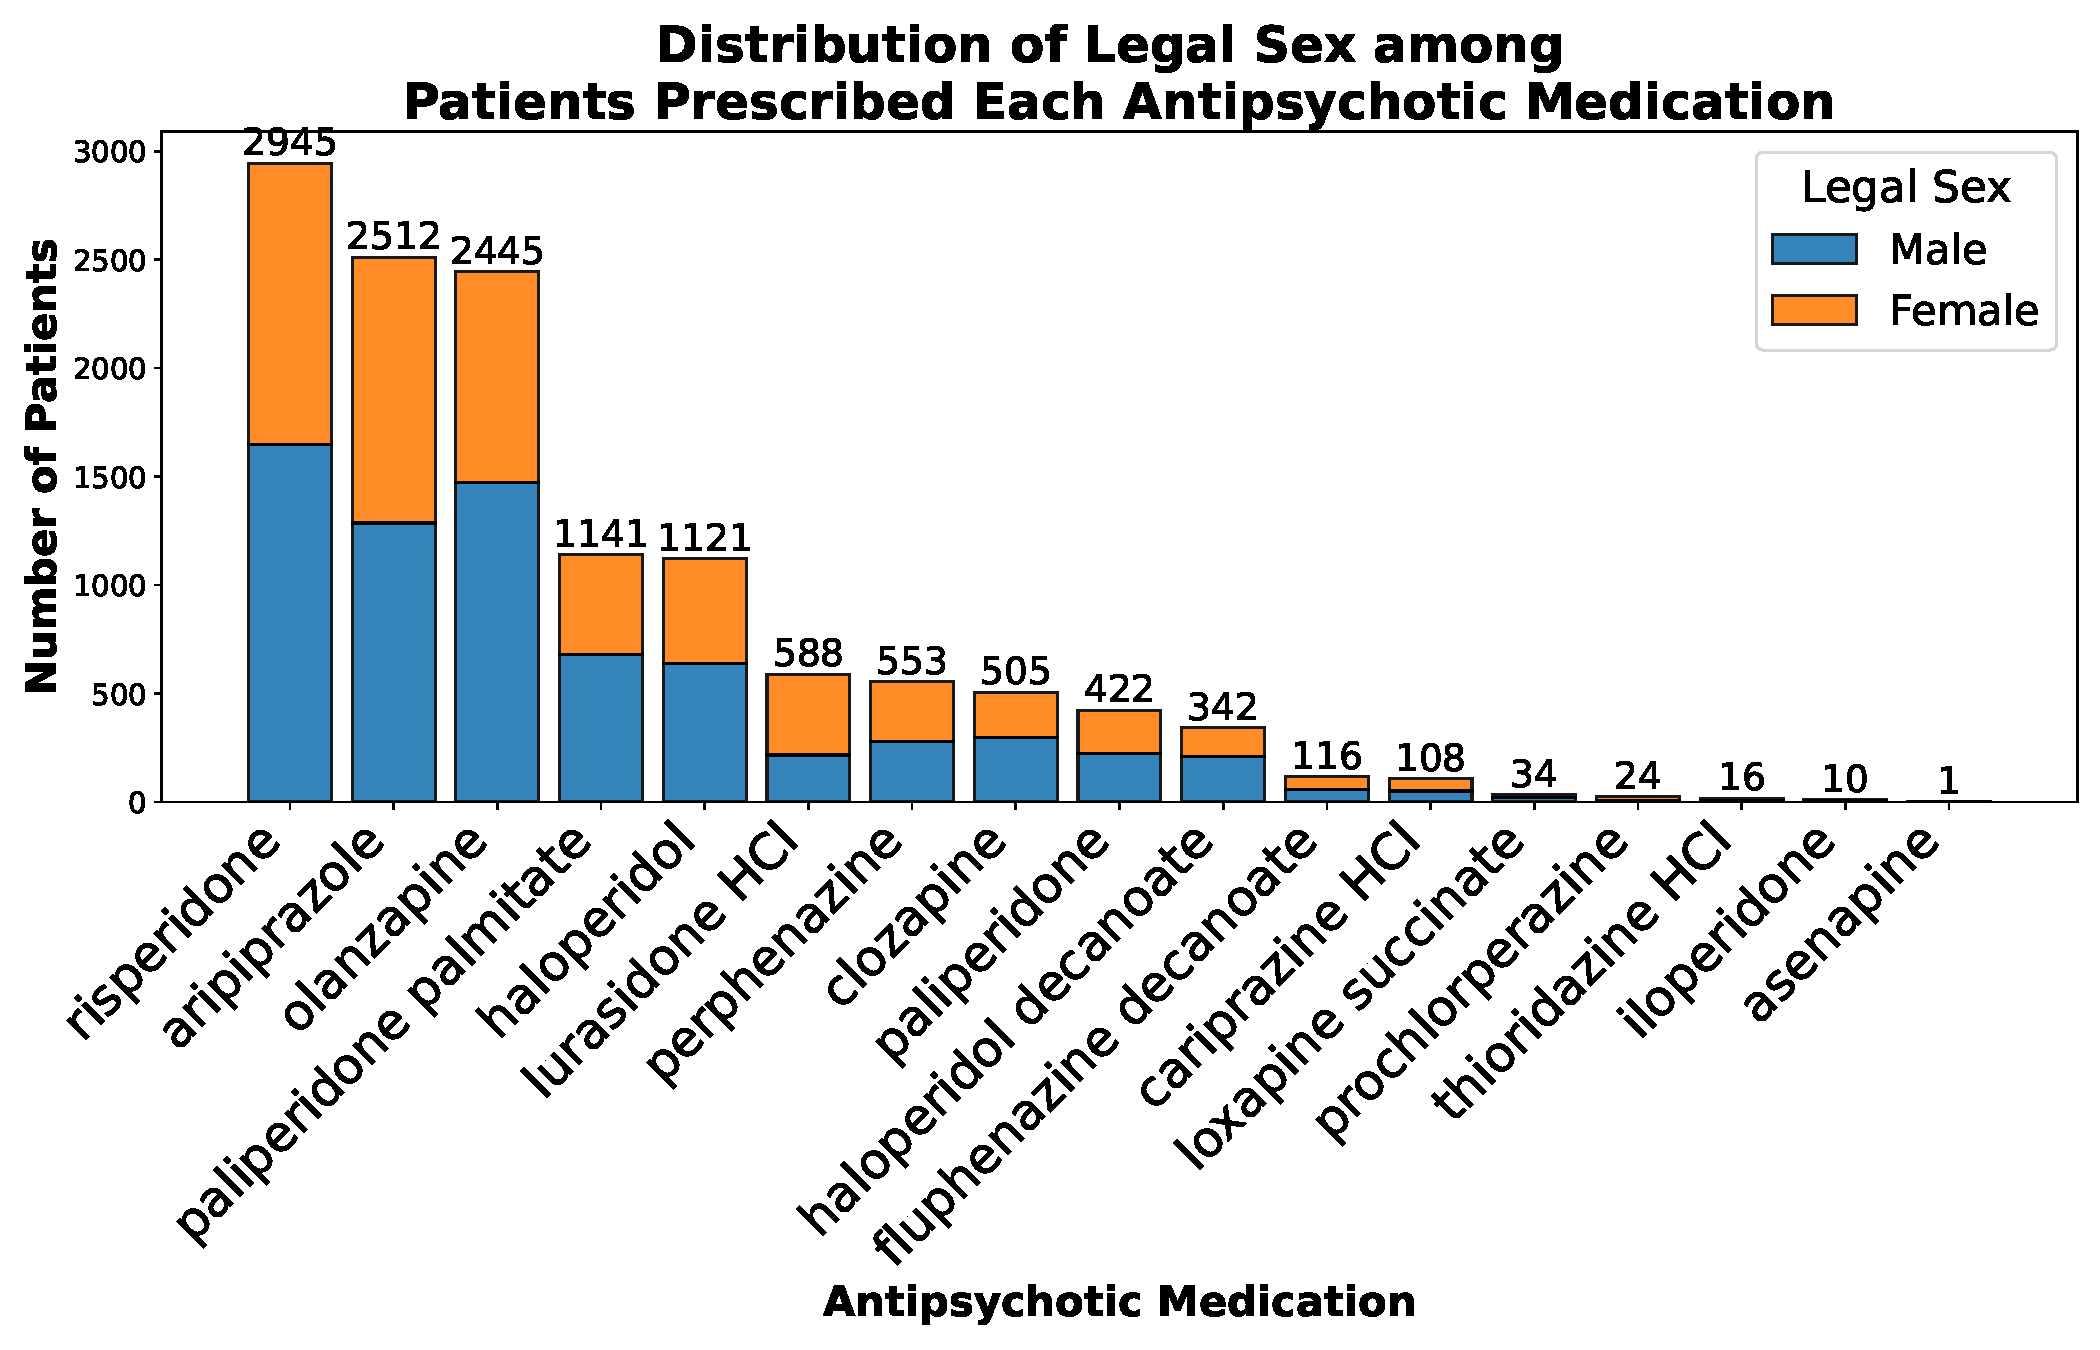
\includegraphics[width=0.458\linewidth]{Figures/Medications/distribution_of_legal_sex_among_patients_prescribed_each_antipsychotic_medication.pdf}}%
    \\
    \subfigure[Race]{\label{fig:medication_race}%
      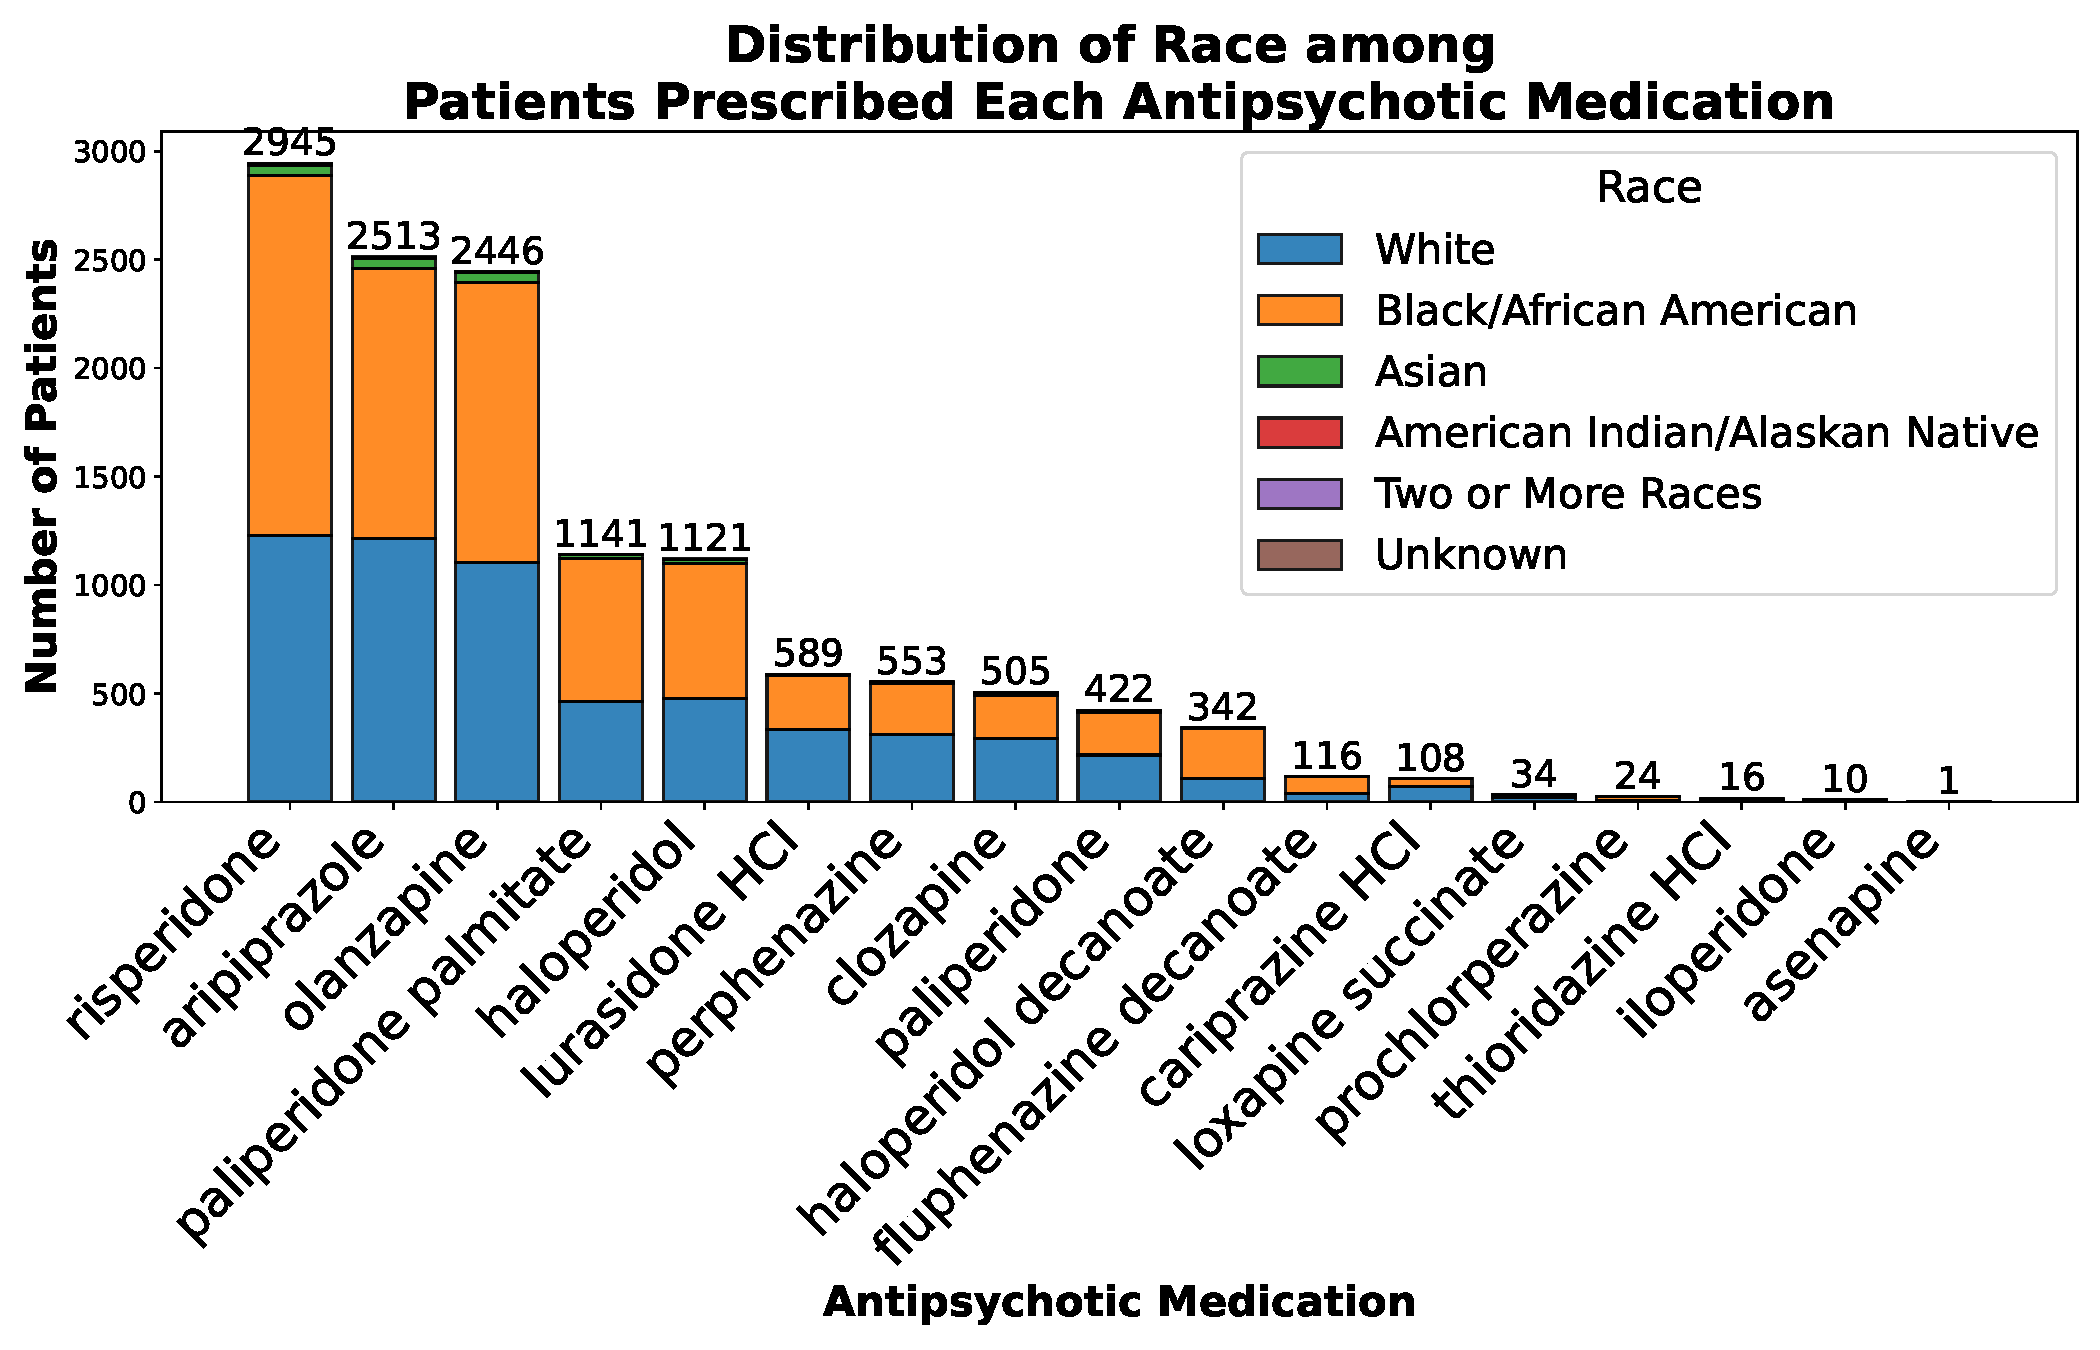
\includegraphics[width=0.458\linewidth]{Figures/Medications/distribution_of_race_among_patients_prescribed_each_antipsychotic_medication.pdf}}%
    \qquad
    \subfigure[Education Level]{\label{fig:medication_education}%
      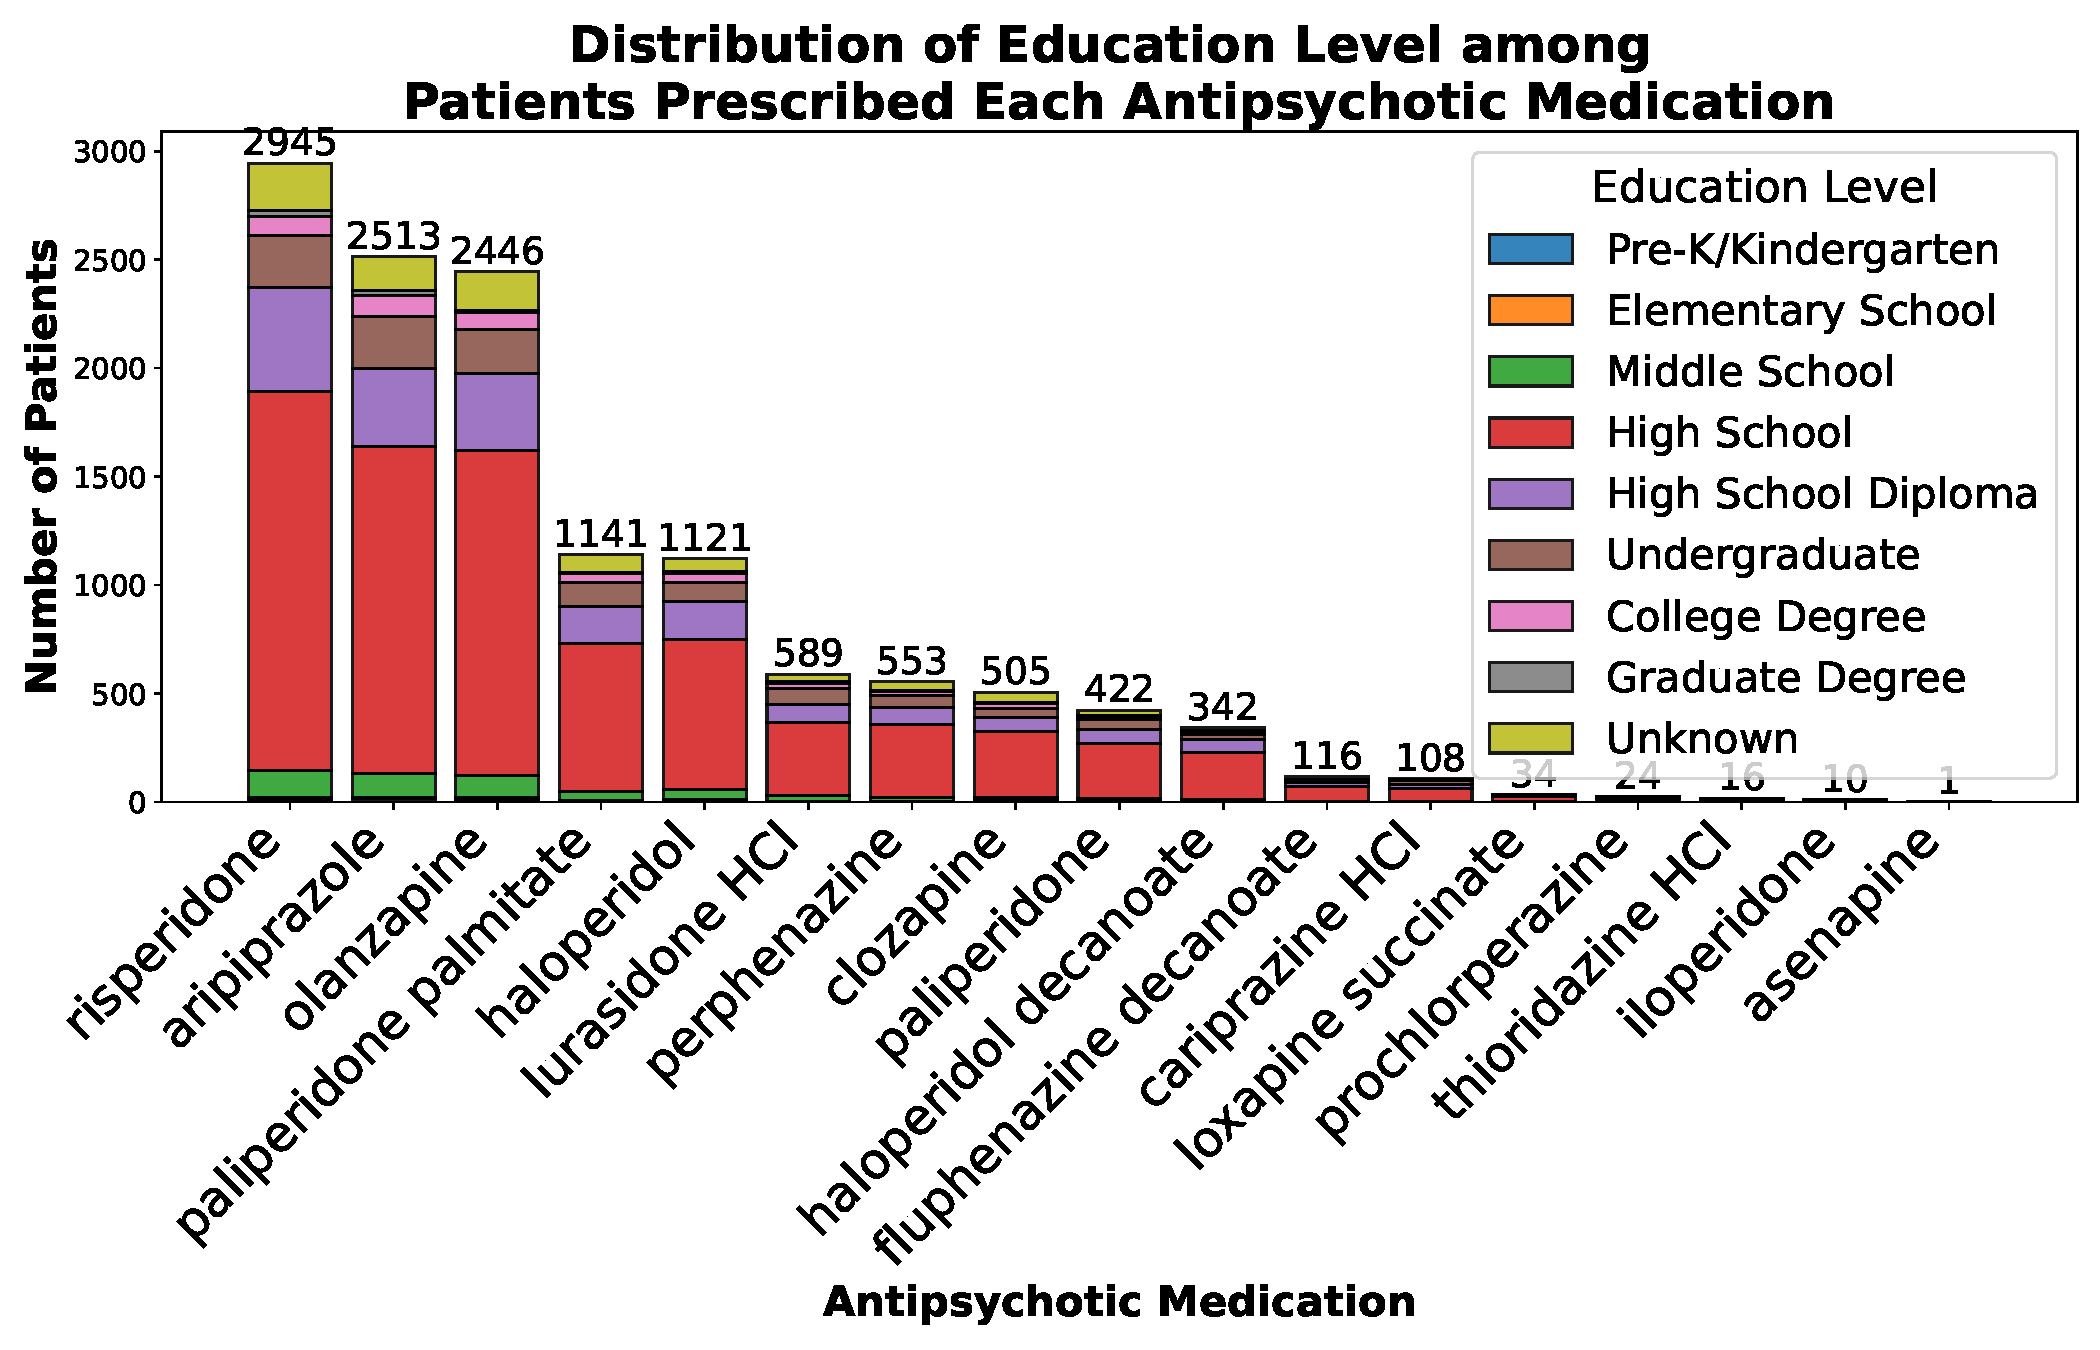
\includegraphics[width=0.458\linewidth]{Figures/Medications/distribution_of_education_level_among_patients_prescribed_each_antipsychotic_medication.pdf}}%
    \\
    \subfigure[Age]{\label{fig:medication_age}%
      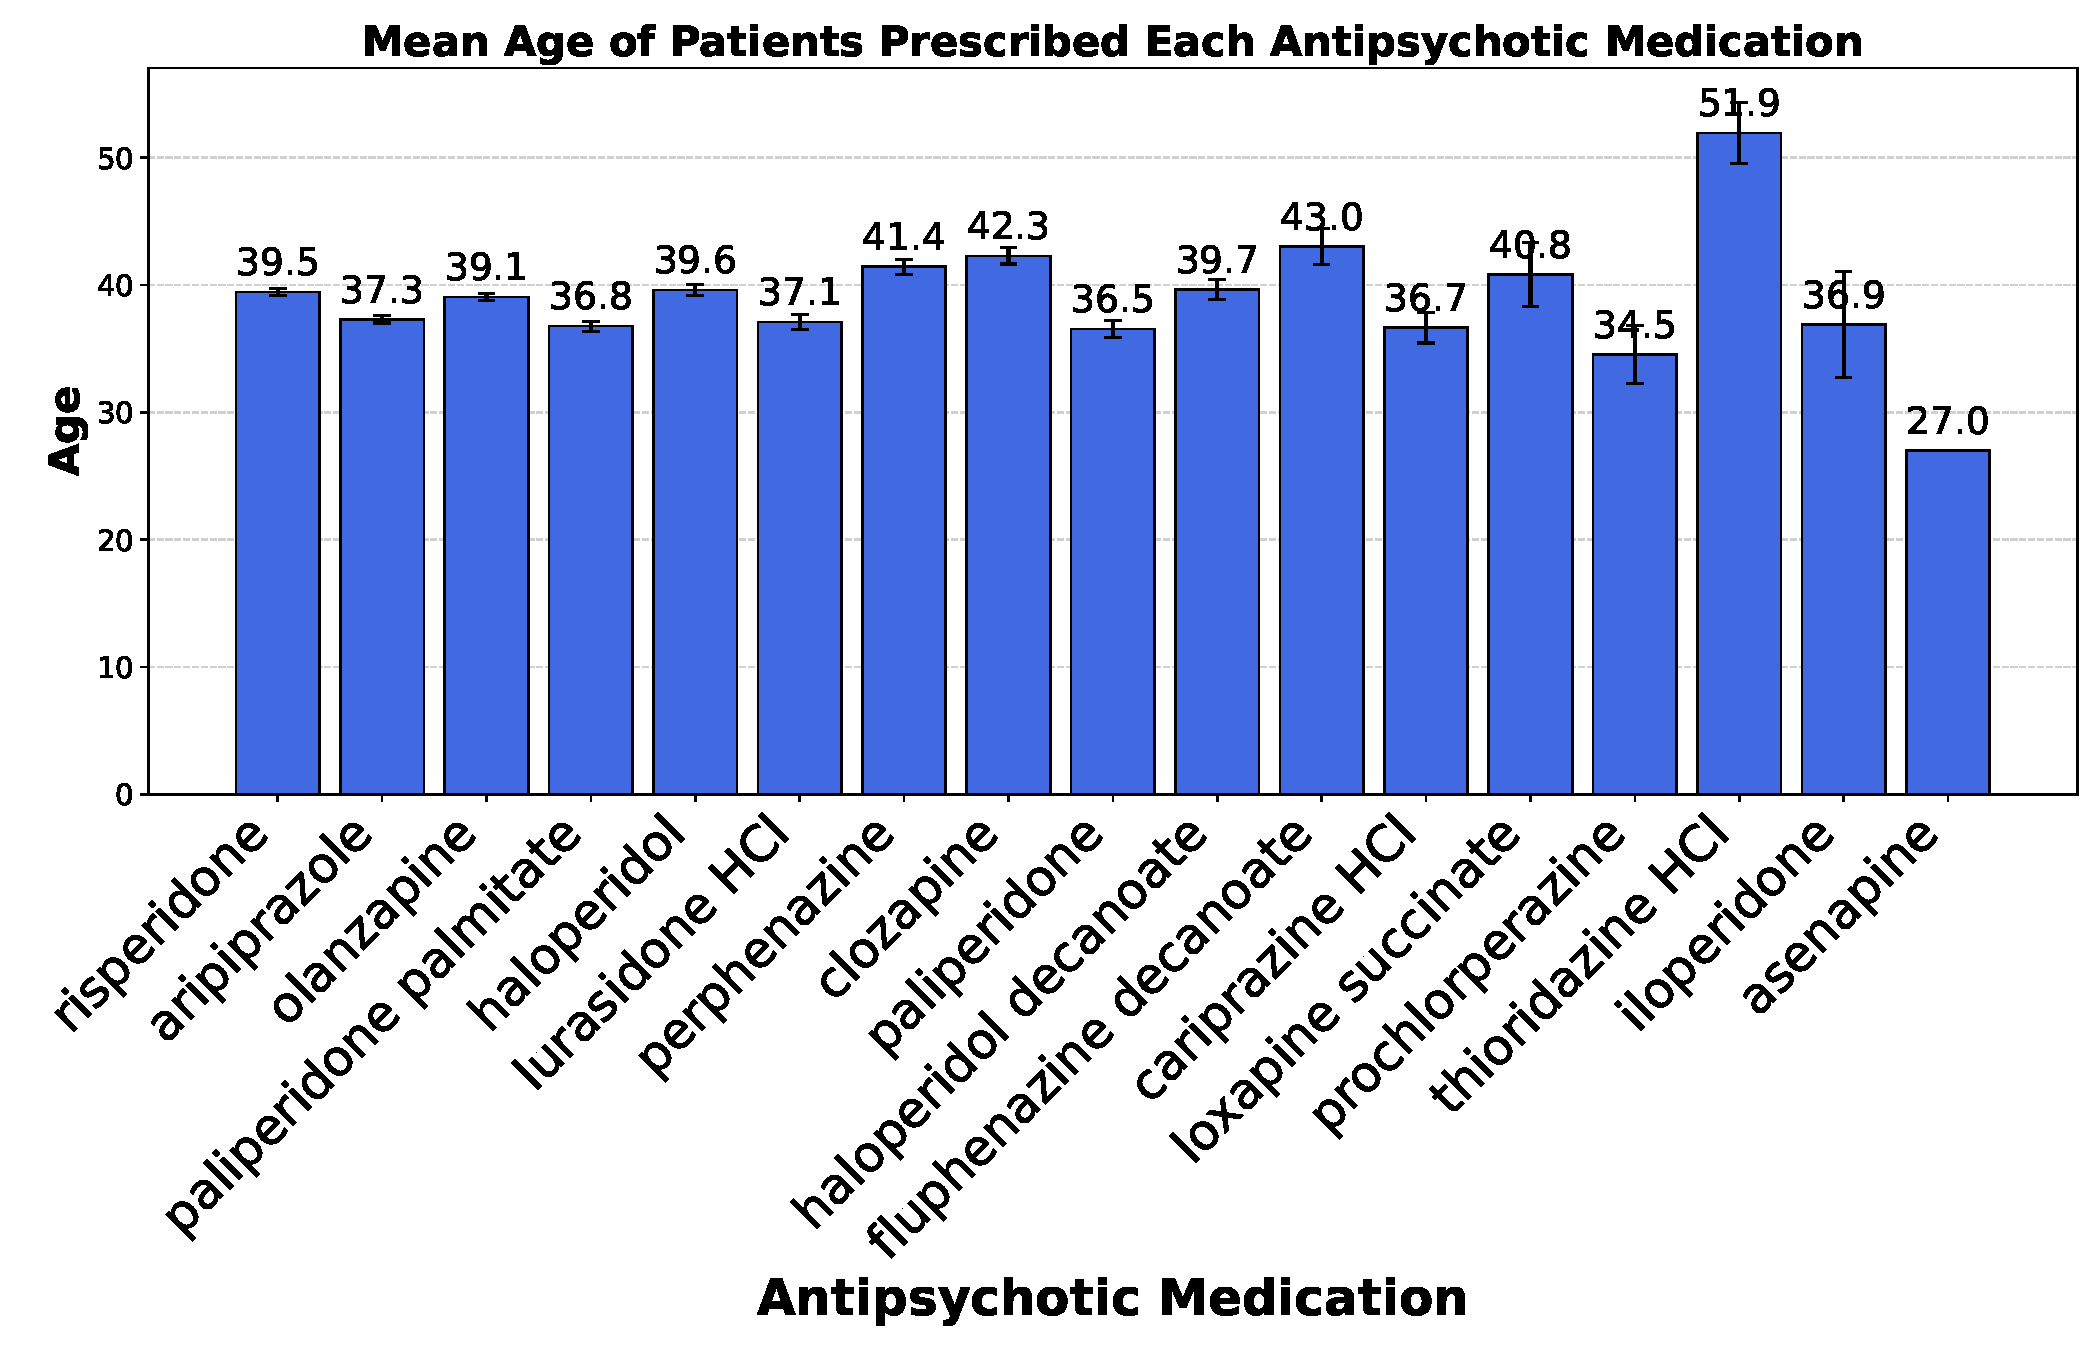
\includegraphics[width=0.458\linewidth]{Figures/Medications/mean_age_of_patients_prescribed_each_antipsychotic_medication.pdf}}%
    \qquad
        \subfigure[Non-Adherence Level]{\label{fig:medication_non_adherence}%
      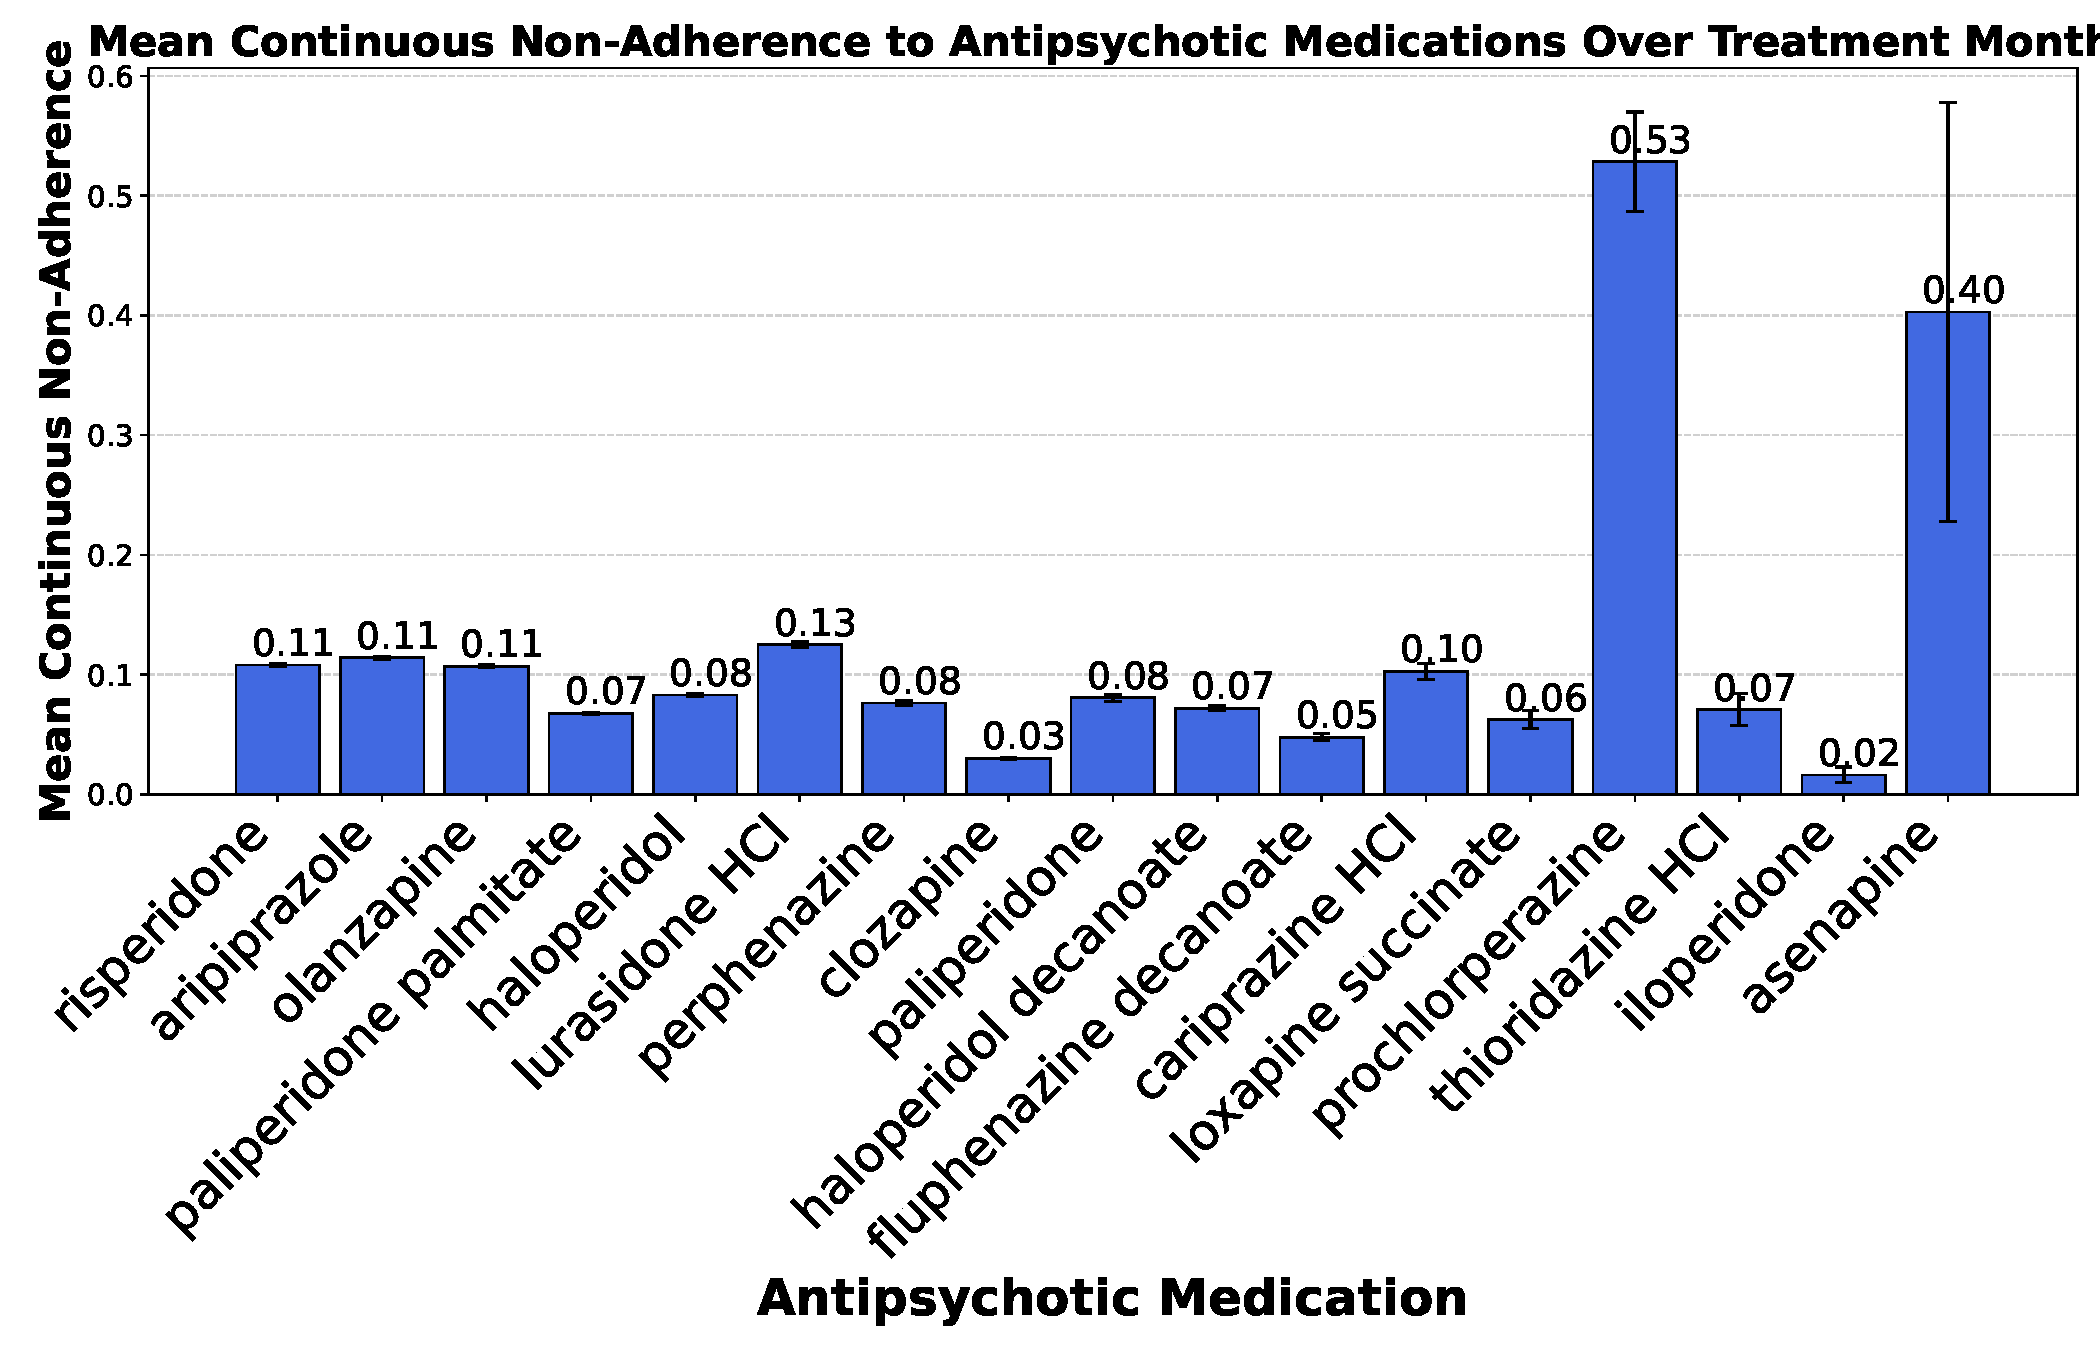
\includegraphics[width=0.458\linewidth]{Figures/Medications/mean_continuous_non_adherence_for_antipsychotics.pdf}}%
  }
\end{figure*}

We examine the usage patterns of the antipsychotic medications within the patient cohort, considering factors such as prevalence of each medication, demographic distribution, adherence behavior, and other relevant characteristics in Figure~\ref{fig:medications}. 
Understanding these patterns provides insights into prescribing trends but also highlights potential challenges in treatment adherence and accessibility across diverse patient populations.
It should be noted that for all subfigure of Figure~\ref{fig:medications}, the x-axis is ordered from left to right based on the frequency of each medication being prescribed to the patients in our cohort with the risperidone being the most prevalent and asenapine being the least prevalent medication in our cohort of study.

Figure~\ref{fig:medication_prevalence} highlights the prevalence of antipsychotic medications in the study cohort. 
Risperidone emerges as the most commonly prescribed medication, with 43.1\% of patients receiving this treatment. 
It is closely followed by aripiprazole (36.8\%) and olanzapine (35.8\%). 
Paliperidone palmitate and haloperidol are also frequently prescribed, though at a lower prevalence of 16.7\% and 6.4\%, respectively. 
Other medications, such as loxapine and asenapine, exhibit minimal usage within the cohort, with fewer than 1\% of patients receiving these prescriptions. 
These results reflect the dominance of specific medications in treatment strategies for psychiatric conditions within this cohort.

Figure~\ref{fig:medication_gender} illustrates the distribution of legal sex among patients prescribed each antipsychotic medication. 
For most medications, the proportion of male patients exceeds that of female patients, consistent with the distribution seen in Appendix~\ref{apd:cohort_demographics}. 
Medications such as risperidone, aripiprazole, and olanzapine, which have the highest overall usage, exhibit similar male-to-female ratios. 
Interestingly, lurasidone HCl and perphenazine show slightly different distributions between the two genders (with the former being more predominant among females), potentially reflecting variations in prescribing practices or differences in the target patient populations for these drugs.

Figure~\ref{fig:medication_race} illustrates the racial demographics of patients prescribed various antipsychotic medications.
Black/African American patients, similar to the demographical composition of our cohort, represent the largest group for most medications, with particularly high representation for risperidone, aripiprazole, and olanzapine.
White patients constitute a sizable proportion of patients for many medications, including risperidone and aripiprazole, where their representation is nearly equal to that of Black/African American patients.
For certain medications, such as haloperidol and paliperidone palmitate, Black/African American patients are the clear majority group, demonstrating variations in prescribing trends.
Patients identifying as Asian, American Indian/Alaskan Native, or Two or More Races are minimally represented across all medications, and the proportion of patients with unknown racial information is similarly low.
These patterns may reflect differences in prescribing practices, patient demographics, or healthcare access within the study cohort.

Figure~\ref{fig:medication_education} shows the distribution of education levels among patients prescribed each antipsychotic medication. 
High school eduation are the most prevalent group for nearly all medications consistent with education level composition of our cohort with high school diploma also represented prominently. 
College education, graduate degree, and lower education levels, such as elementary or middle school, are much less frequent among the cohort. 
We do not see a particular trend suggesting a possible direct association between education level and medication type in our cohort.

Figure~\ref{fig:medication_age} presents the mean age of patients prescribed each antipsychotic medication. 
The mean age for most medications falls within the range of 36 to 43 years, consistent with the typical age of onset for psychiatric conditions treated with antipsychotics. 
Interestingly, patients prescribed thioridazine HCl tend to be older, with a mean age exceeding 50 years. 
In contrast, asenapine is associated with a significantly younger patient population, with a mean age of 27 years. 
These age differences may reflect the specific clinical indications or prescribing patterns for these medications.

Figure~\ref{fig:medication_non_adherence} explores the mean continuous non-adherence scores for each antipsychotic medication. 
Most medications, including risperidone, aripiprazole, and olanzapine, have low non-adherence scores (below 0.15), indicating relatively high adherence levels. 
However, certain medications, such as prochlorperazine and asenapine, exhibit markedly higher non-adherence scores of 0.53 and 0.40, respectively. 
It should be noted that these two medications are among the least frequent medications in our study and hence there is high uncertainty involved with their adherence levels in our analysis. 
Nevertheless, these preliminary findings highlight some challenges associated with maintaining adherence for specific medications, potentially due to side effects, dosing regimens, or other factors influencing patient compliance. 
Future research could focus on understanding the reasons behind these adherence disparities, including the role of patient characteristics, medication accessibility, and the severity of side effects. 

\vspace{-0.75em}
\subsection{Predictability of the Risk Scores in Our Data}
\label{apd:risk_score_evaluations}
\vspace{-0.25em}

\begin{figure}[htbp]
\floatconts
  {fig:roc_predictability_of_risks}
  {\caption{ROC curves assessing the accuracy of county-provided risk scores for predicting adverse events within 12 months. The AUC quantifies performance for (a) \textcolor{orange}{Involuntary Hospitalization} (b) \textcolor{red}{Jail Stay} and (c) \textbf{Mortality}.}}
  {%
    \subfigure[Involuntary Hospitalization]{\label{fig:roc_302_risk}%
      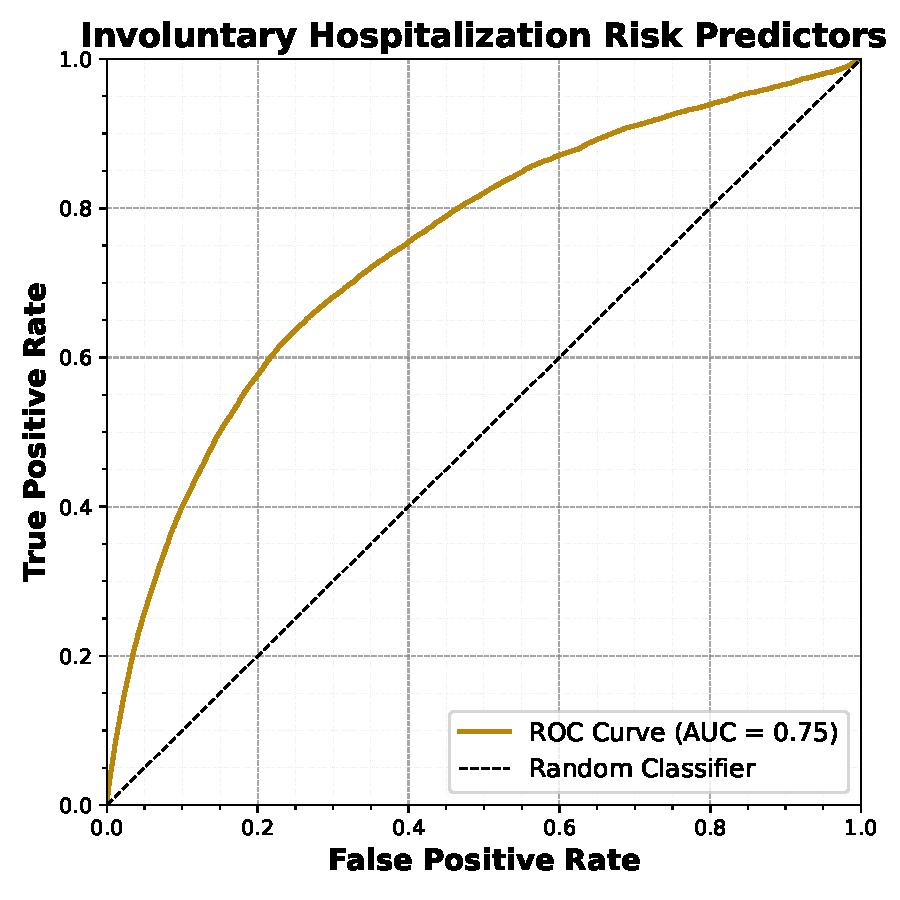
\includegraphics[width=.67\linewidth]{Figures/roc_curve_involuntary_hospitalization_risk.pdf}}%
    \\
    \subfigure[Jail Stay]{\label{fig:roc_jail_risk}%
      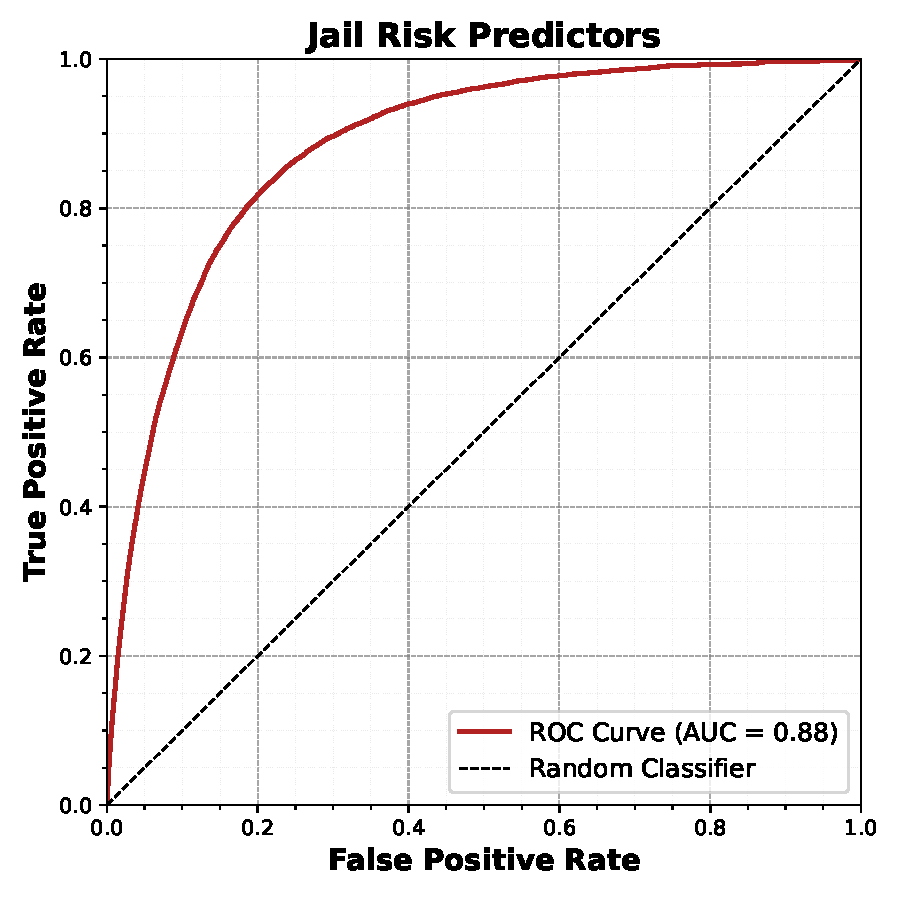
\includegraphics[width=.67\linewidth]{Figures/roc_curve_jail_risk.pdf}}
    \\
    \subfigure[Mortality]{\label{fig:roc_death_risk}%
      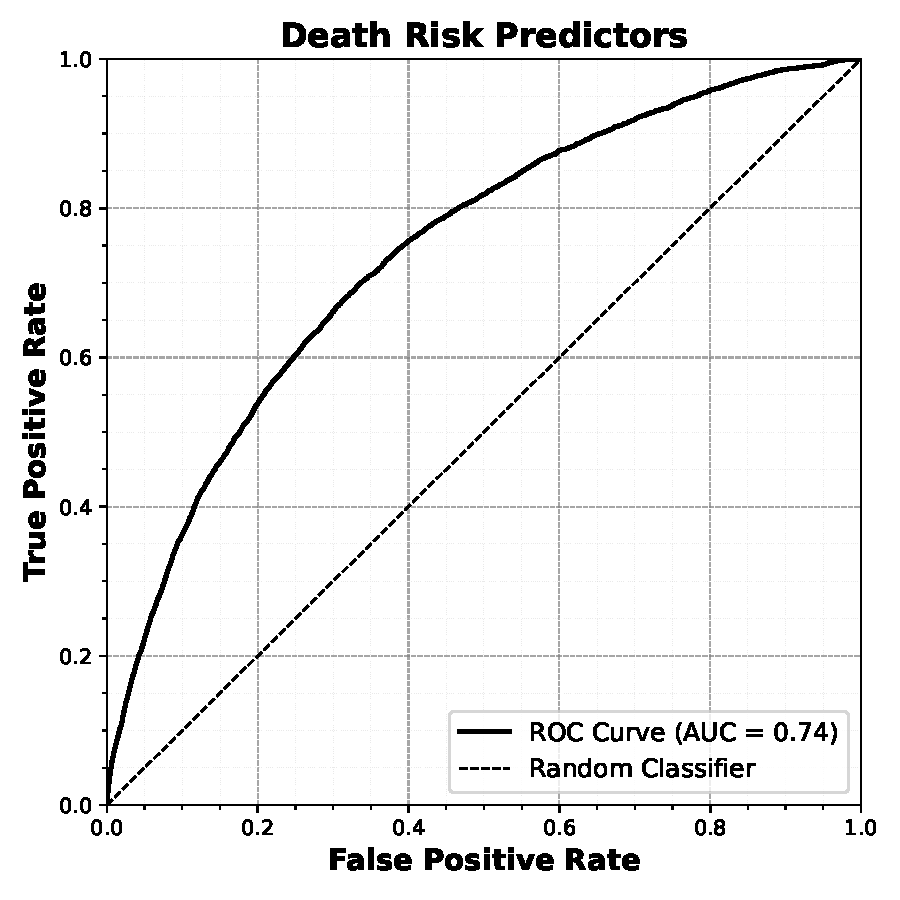
\includegraphics[width=.67\linewidth]{Figures/roc_curve_death_risk.pdf}}
  }
\end{figure}

To evaluate the predictive accuracy of county-provided risk scores described in Section~\ref{sec:methods_data} in our data, we assess their ability to predict adverse events within 12 months.
The county-provided risk scores that we evaluate correspond to probabilities of three specific adverse events that we have access to: involuntary hospitalization, jail stay, and mortality.
Using ground truth outcomes available in our dataset, we compute Receiver Operating Characteristic (ROC) curves for each risk score and quantify performance using the Area Under the Curve (AUC).

Figure~\ref{fig:roc_predictability_of_risks} presents the ROC curves for the three adverse events.
For involuntary hospitalization (Figure~\ref{fig:roc_302_risk}), the risk score achieves an AUC of 0.75, indicating moderate predictive performance.
The jail stay risk score (Figure~\ref{fig:roc_jail_risk}) performs better, with an AUC of 0.88, reflecting strong discrimination between individuals at higher versus lower risk.
In contrast, the mortality risk score (Figure~\ref{fig:roc_death_risk}) achieves an AUC of 0.74, comparable to involuntary hospitalization, but still reflecting only moderate predictive accuracy.

These results suggest that while the county-provided risk scores capture some signal related to adverse events, their predictive performance varies significantly across outcomes.
Jail stay predictions are relatively reliable, whereas involuntary hospitalization and mortality scores exhibit room for improvement.
These results indicate that the county-provided risk scores capture some signal related to adverse events, though their performance varies across outcomes.
In this study, we incorporate these risk scores as covariates in our models, where they serve as proxies for unmeasured confounders.
Their inclusion helps to isolate the Average Treatment Effect (ATE) of non-adherence by accounting for confounding factors that would otherwise remain unobserved.